\documentclass[12pt]{article}
\usepackage{spikey}
\usepackage{amsmath}
\usepackage{amssymb}
\usepackage{soul}
\usepackage{float}
\usepackage{graphicx}
\usepackage{hyperref}
\usepackage{xcolor}
\usepackage{chngcntr}
\usepackage{centernot}
\usepackage{datetime}
\usepackage[shortlabels]{enumitem}
\usepackage{booktabs}

% Set font.
%\usepackage{fontspec}
 
%\setmainfont{Times New Roman}
%\usepackage{mathptmx}
%\usepackage[MnSymbol]{mathspec}
%\setallmainfonts{Times New Roman}

\usepackage[margin=1truein]{geometry}
\usepackage{setspace}
\linespread{1.5}

\counterwithin{equation}{section}
\counterwithin{theorem}{section}
\counterwithin{lemma}{section}
\counterwithin{corollary}{section}
\counterwithin{proposition}{section}
\counterwithin{remark}{section}
\counterwithin{example}{section}
\counterwithin{definition}{section}

% Bib package
\usepackage{apacite}

\title{Forecasting Crude Oil Returns using News Sentiment and Machine Learning \footnote{Compile Date: \currenttime\ \today}}

\author{Tianyu Du \footnote{\texttt{tianyu.du@mail.utoronto.ca}}}

\begin{document}
	\maketitle
	\tableofcontents
	\newpage
	\section{Introduction}
	
	\section{Data}
	\paragraph{}In order to identify the predictive power of sentiment data on crude oil returns, this study involves three major datasets, a the daily spot price of crude oil at the West Texas Intermediate (WTI) from which returns are computed, ii) a news sentiment dataset from Ravenpack News Analytics (RPNA), and iii) other macroeconomic indicators proxying the overall economic background.

	\subsection{The West Texas Intermediate (WTI) Crude Oil Dataset}
%	\paragraph{}West Texas Intermediate market spot price (coded as DCOILWTICO in the st. Louis Federal Reserve Economic Data) has been the most commonly used price for crude oil in current literature. The dataset retrieved from the Federal Reserve Bank of St. Louis is measured on a daily level and spans from January 1986 up to the present day (citation: data series). Because of the limited availability of the RavenPack dataset, this paper focuses only on crude oil prices after January 1, 2000. Analysis of the crude oil market (citation: 40-year paper) shows the spot price is higuly responsive to news and other macroeconomic shocks, which is exactly the tricky part of forecasting financial time series. If the proposed forecasting pipeline performs well on the crude dataset, such a pipeline is conceivably promising on other datasets as well.
	
%	\par Almost all financial time series suffers from missing data problem, so is the crude oil dataset. Much existing research studying stock market datasets simply drop missing values. Instead, this paper uses an autoregressive integrated moving average (ARIMA) model to interpolate and fill missing data, so that the time gap between two consecutive observations is exactly one trading day. 

	\subsection{Summary Statistics of Crude Oil Dataset}
	\begin{figure}[H]
		\small
		\centering
		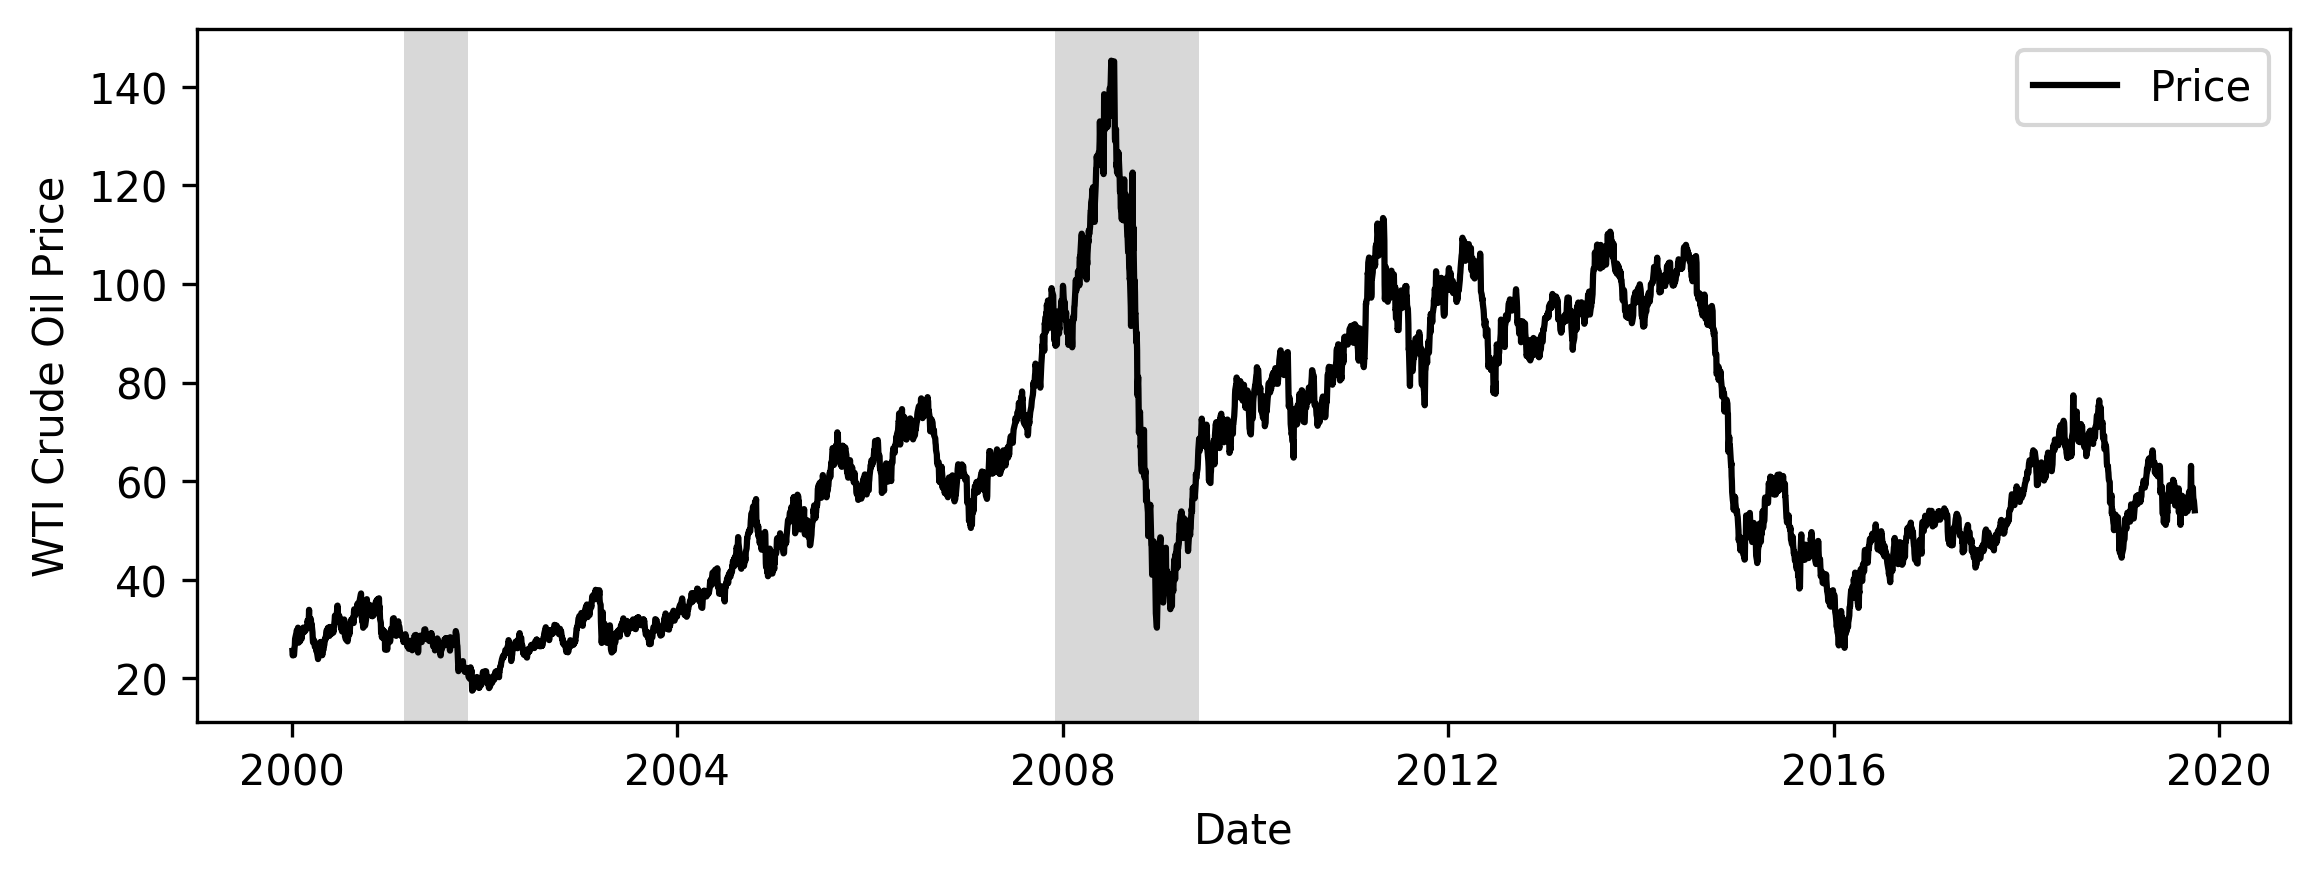
\includegraphics[width=\linewidth]{figures/wti_summary/prices.png}
		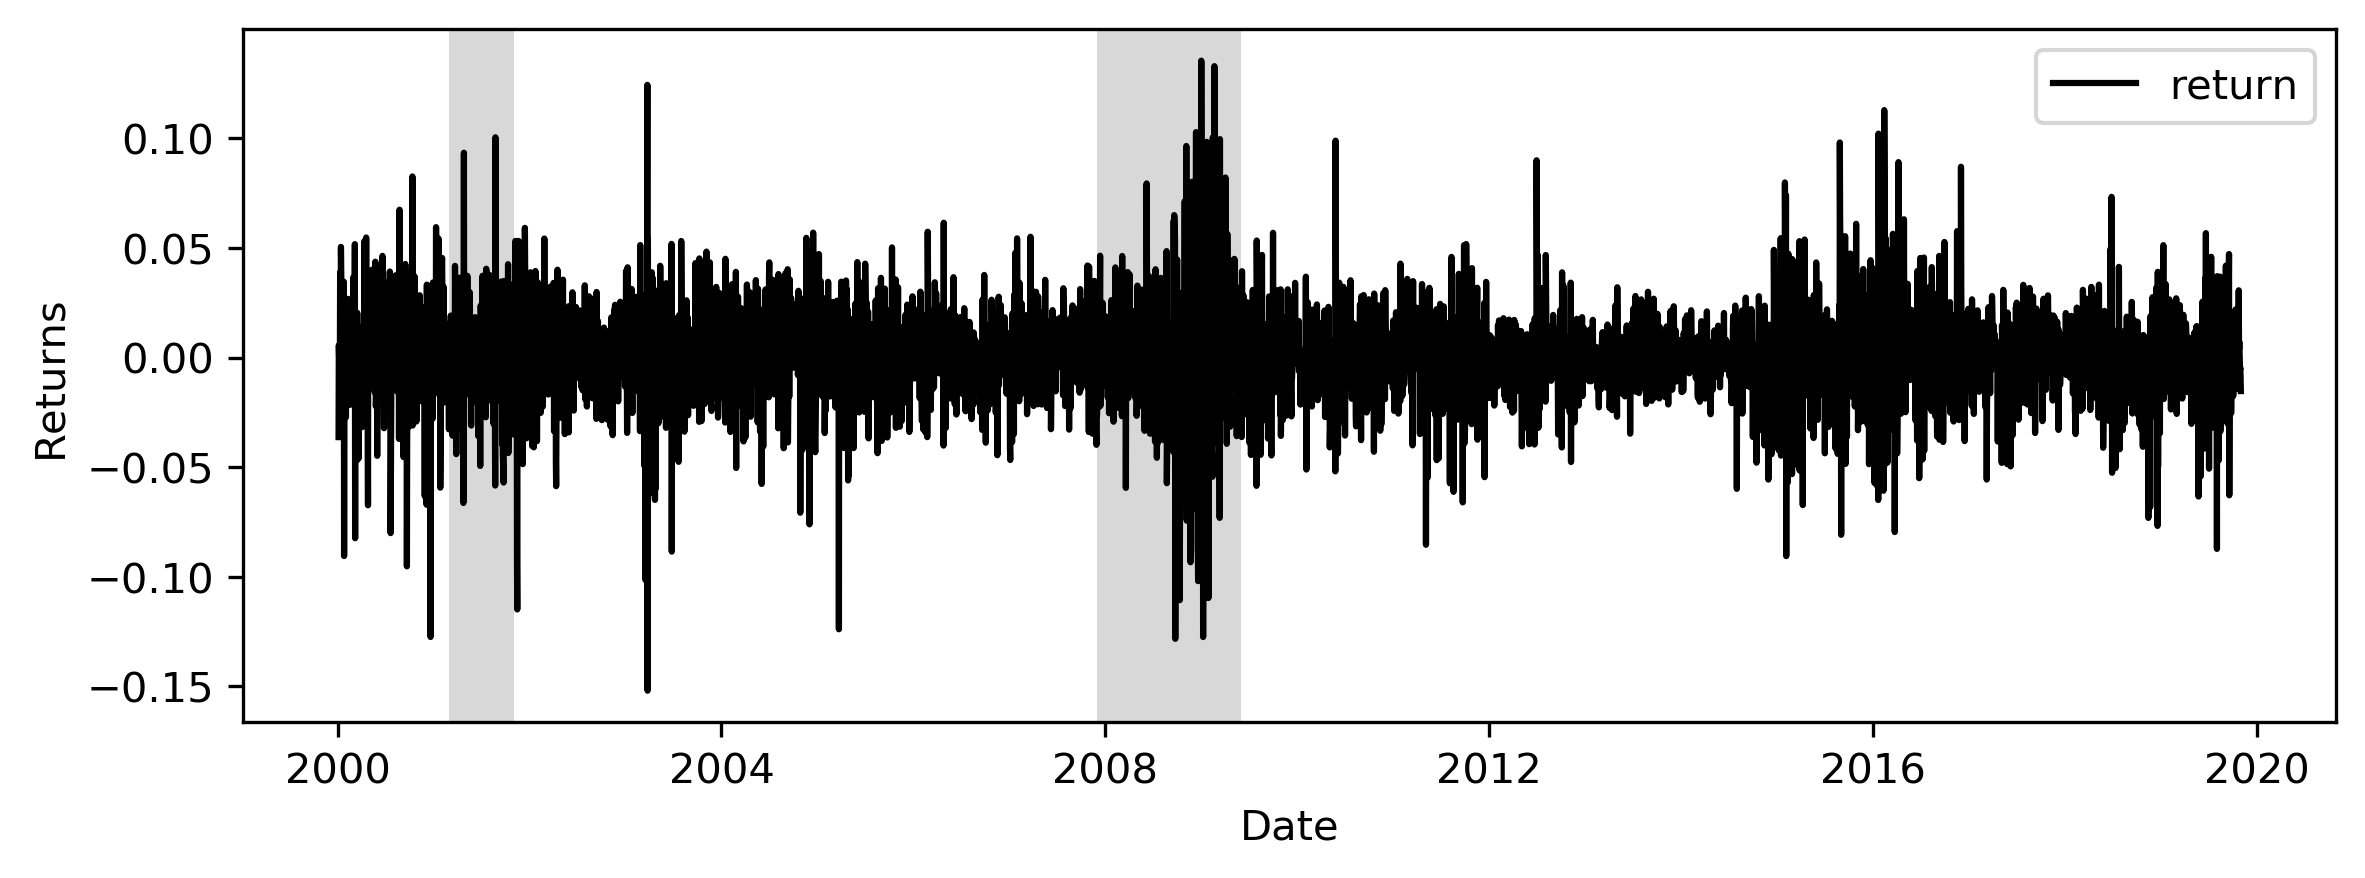
\includegraphics[width=\linewidth]{figures/wti_summary/returns.png}
		\caption{Crude oil prices and returns between January 1, 2000 and September 30, 2019. Shaded areas indicate U.S. recessions.}
	\end{figure}

	\par From the \textbf{the table below} we can see that the mean returns for crude oil are around zero year by year. During periods of recessions (March 2001 to November 2001 and December 2007 to June 2009), the data exhibited negative mean returns as well as relatively high standard deviations.
	\begin{table}[H]
		\small
		\centering
		\begin{tabular}{l|c c c c c c c c c}
			\toprule
			Year & Num. Obs. & Mean & Median & Std. & Min & Max & ACF(1) & ACF(3) & ACF(5) \\
			\midrule
			2000 & 249 & 0.000 & 0.004 & 0.029 & -0.127 & 0.083 & 0.012 & -0.007 & 0.126 \\
			2001 & 250 & -0.001 & -0.001 & 0.029 & -0.171 & 0.101 & 0.024 & -0.005 & -0.037 \\
			2002 & 250 & 0.002 & 0.002 & 0.021 & -0.062 & 0.060 & -0.030 & -0.008 & -0.014 \\
			2003 & 250 & 0.000 & 0.002 & 0.028 & -0.152 & 0.124 & -0.133 & 0.096 & -0.097 \\
			2004 & 249 & 0.001 & 0.003 & 0.023 & -0.076 & 0.059 & -0.074 & 0.019 & -0.036 \\
			2005 & 251 & 0.001 & 0.002 & 0.022 & -0.124 & 0.084 & -0.085 & -0.083 & -0.109 \\
			2006 & 249 & -0.000 & 0.001 & 0.018 & -0.049 & 0.062 & 0.002 & 0.008 & -0.030 \\
			2007 & 252 & 0.002 & 0.001 & 0.019 & -0.047 & 0.055 & -0.103 & 0.000 & 0.069 \\
			2008 & 253 & -0.003 & -0.001 & 0.039 & -0.128 & 0.164 & 0.008 & 0.165 & -0.259 \\
			2009 & 252 & 0.002 & 0.002 & 0.034 & -0.127 & 0.133 & -0.034 & 0.096 & -0.022 \\
			2010 & 252 & 0.001 & 0.000 & 0.019 & -0.052 & 0.099 & 0.051 & -0.071 & 0.057 \\
			2011 & 252 & 0.000 & 0.001 & 0.022 & -0.085 & 0.086 & 0.027 & -0.003 & -0.087 \\
			2012 & 252 & -0.000 & 0.001 & 0.016 & -0.048 & 0.090 & -0.154 & 0.034 & 0.120 \\
			2013 & 252 & 0.000 & 0.001 & 0.011 & -0.035 & 0.032 & 0.045 & -0.073 & -0.153 \\
			2014 & 252 & -0.002 & -0.001 & 0.016 & -0.111 & 0.049 & -0.209 & 0.054 & -0.042 \\
			2015 & 252 & -0.001 & -0.004 & 0.029 & -0.091 & 0.098 & -0.113 & -0.106 & -0.021 \\
			2016 & 252 & 0.001 & 0.000 & 0.031 & -0.080 & 0.113 & 0.006 & -0.040 & 0.078 \\
			2017 & 250 & 0.000 & 0.003 & 0.016 & -0.056 & 0.033 & -0.017 & -0.017 & 0.076 \\
			2018 & 249 & -0.001 & 0.001 & 0.020 & -0.077 & 0.073 & -0.103 & -0.056 & 0.011 \\
			2019 & 187 & 0.001 & 0.001 & 0.023 & -0.087 & 0.142 & -0.090 & -0.039 & 0.123 \\
			\midrule
			Total & 4955 & 0.000 & 0.001 & 0.024 & -0.171 & 0.164 & -0.035 & 0.021 & -0.024 \\
			\bottomrule
		\end{tabular}
		\caption{Summary Statistics for Crude Oil Returns in each Year. Note that this dataset only include nine months of 2019.}
	\end{table}
	
	\begin{figure}[H]
		\small
		\centering
		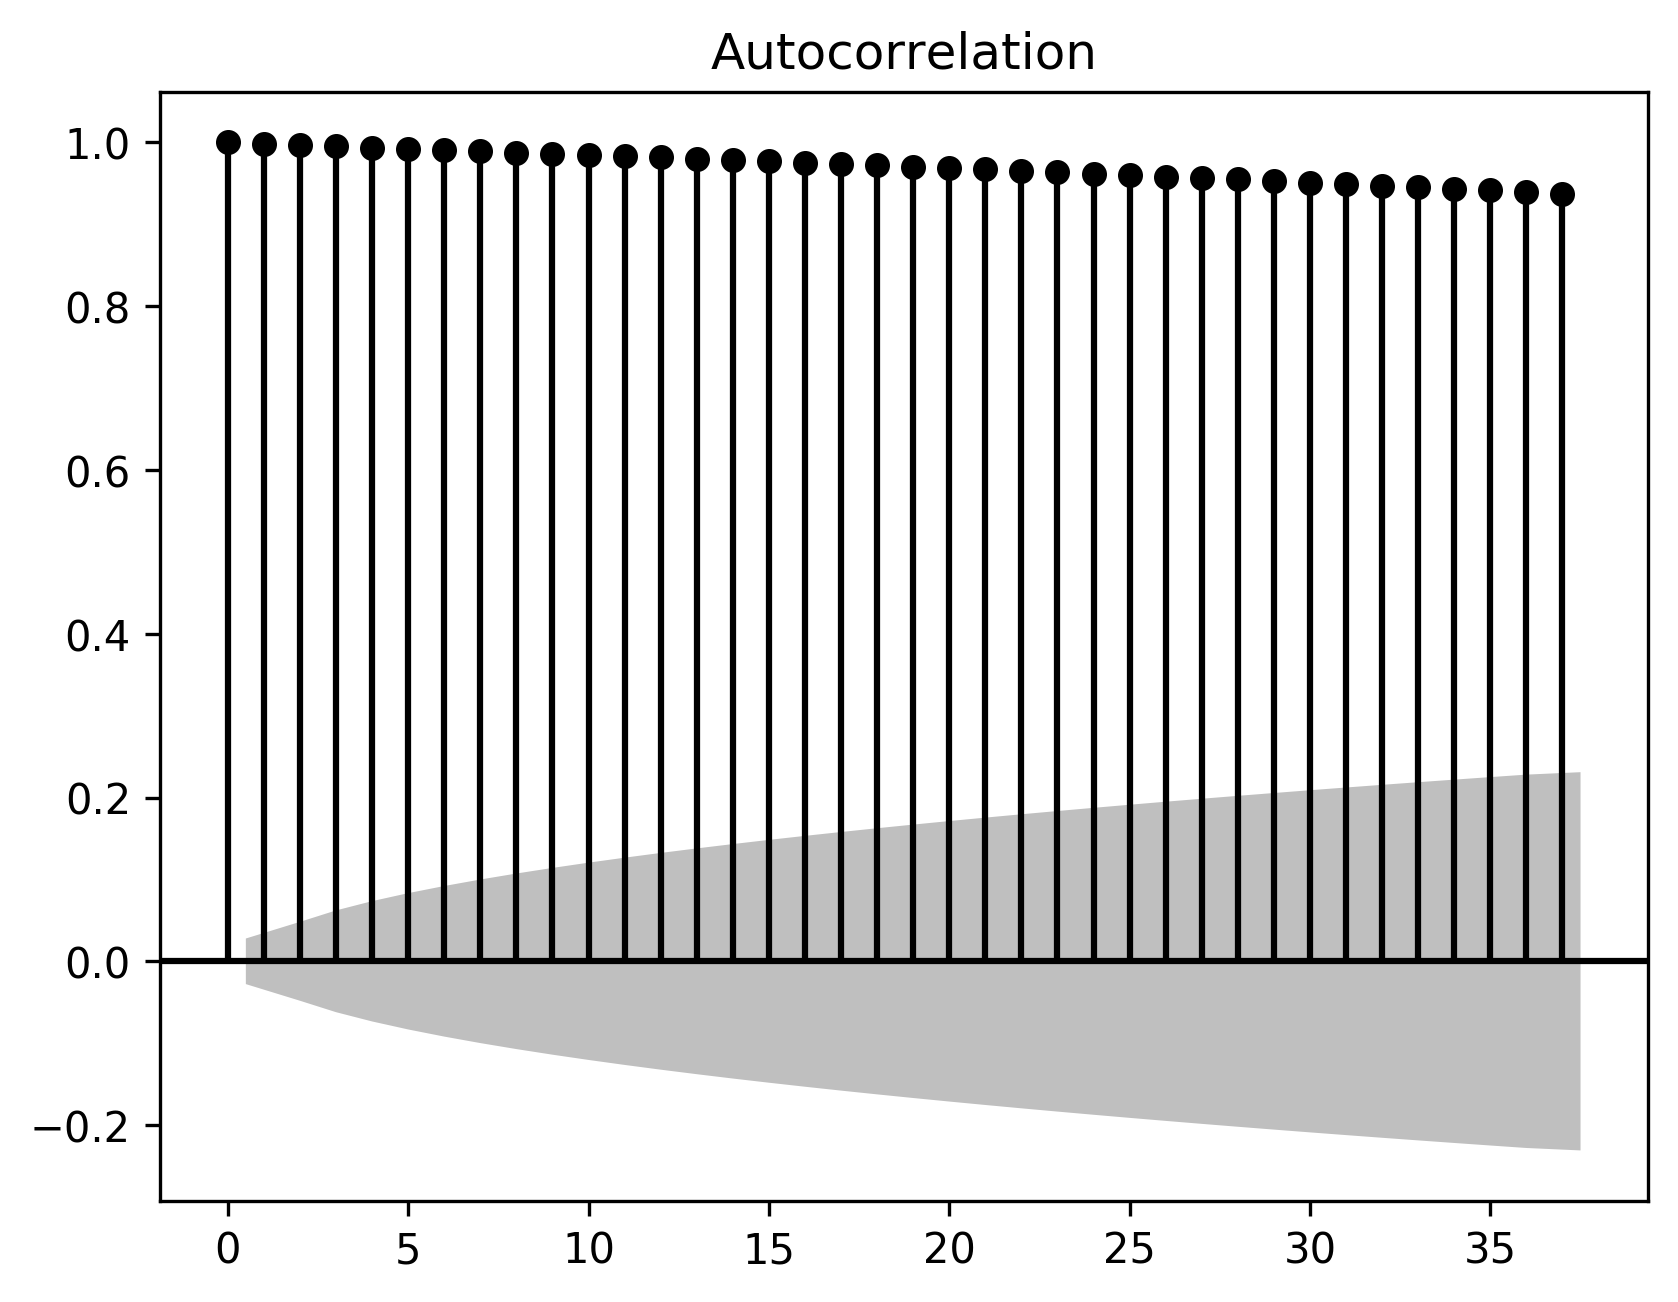
\includegraphics[width=0.45\linewidth]{figures/wti_summary/prices_acf.png}
		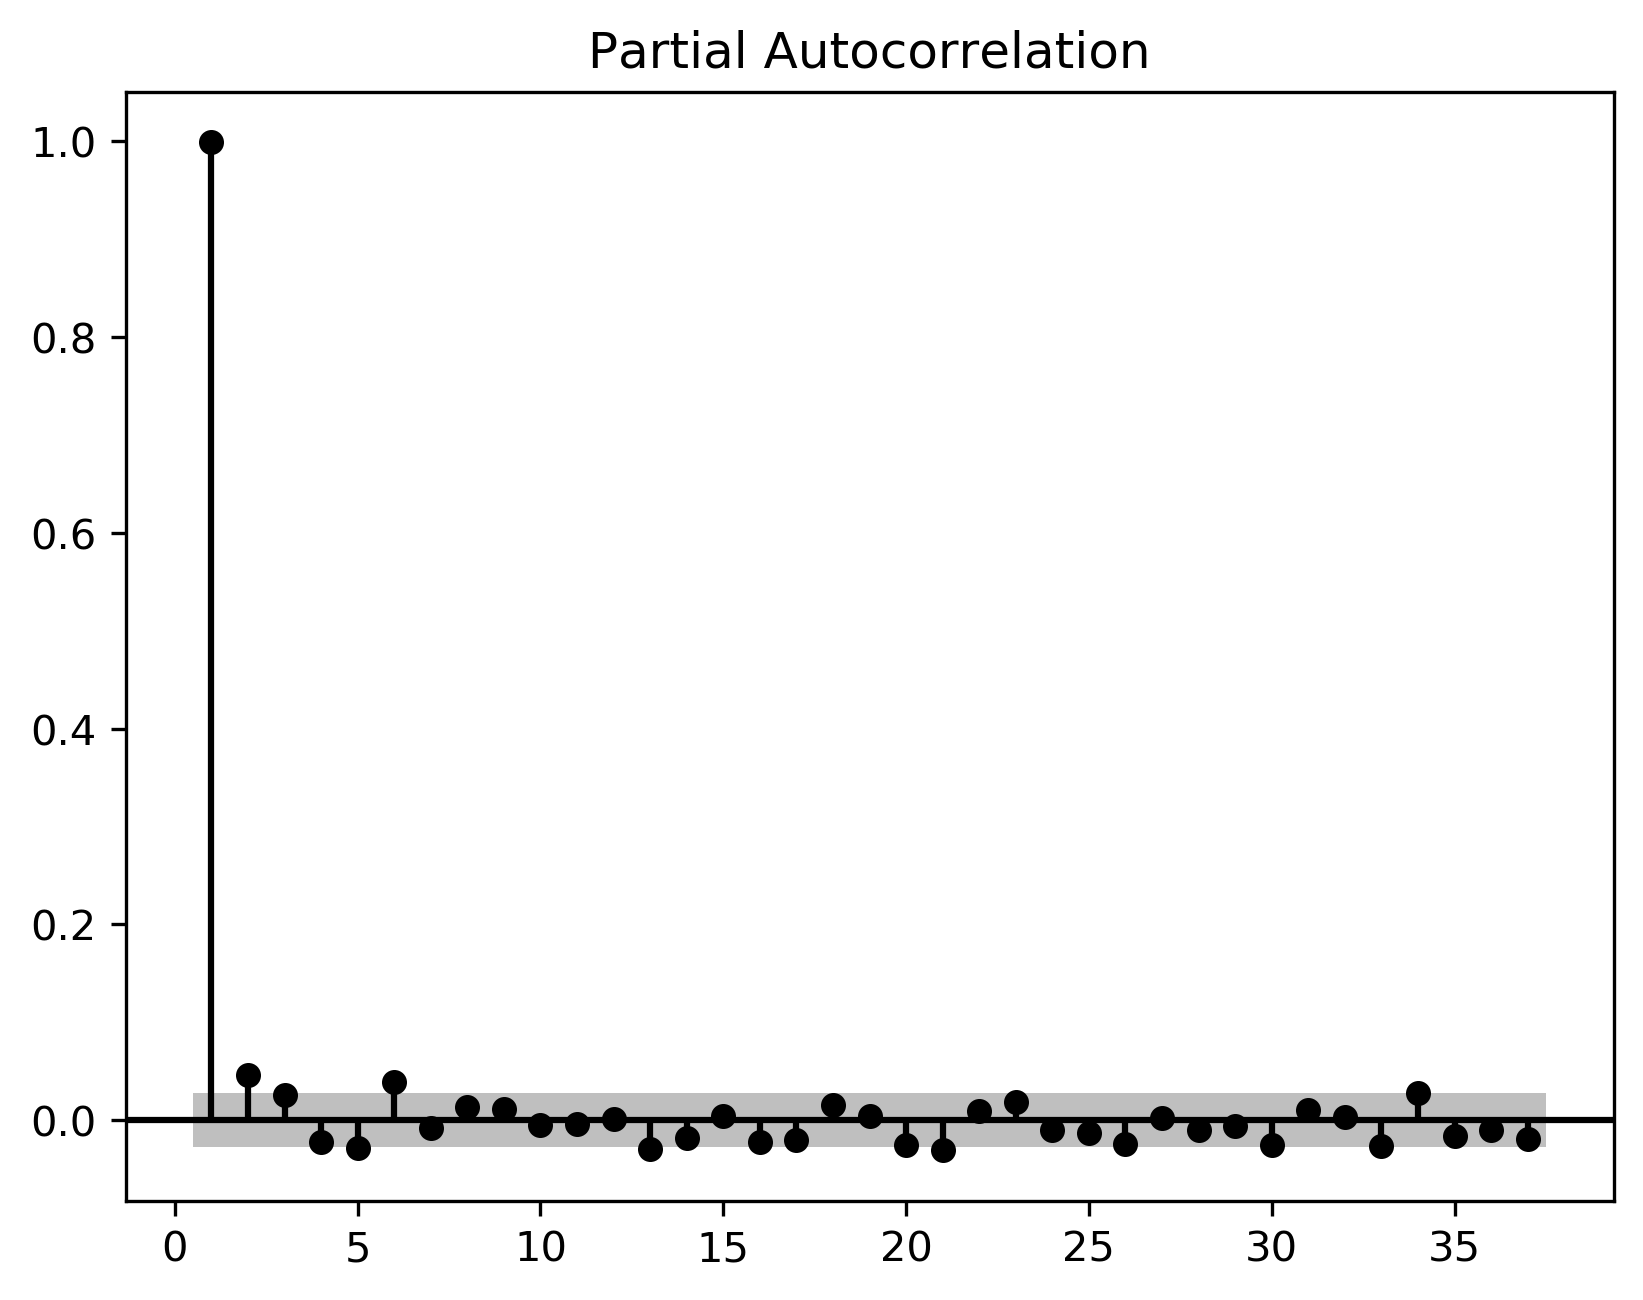
\includegraphics[width=0.45\linewidth]{figures/wti_summary/prices_pacf.png}
		\caption{ACF and PACF for Crude Oil Prices (January 2000 to September 2019)}
	\end{figure}

	\begin{figure}[H]
		\small
		\centering
		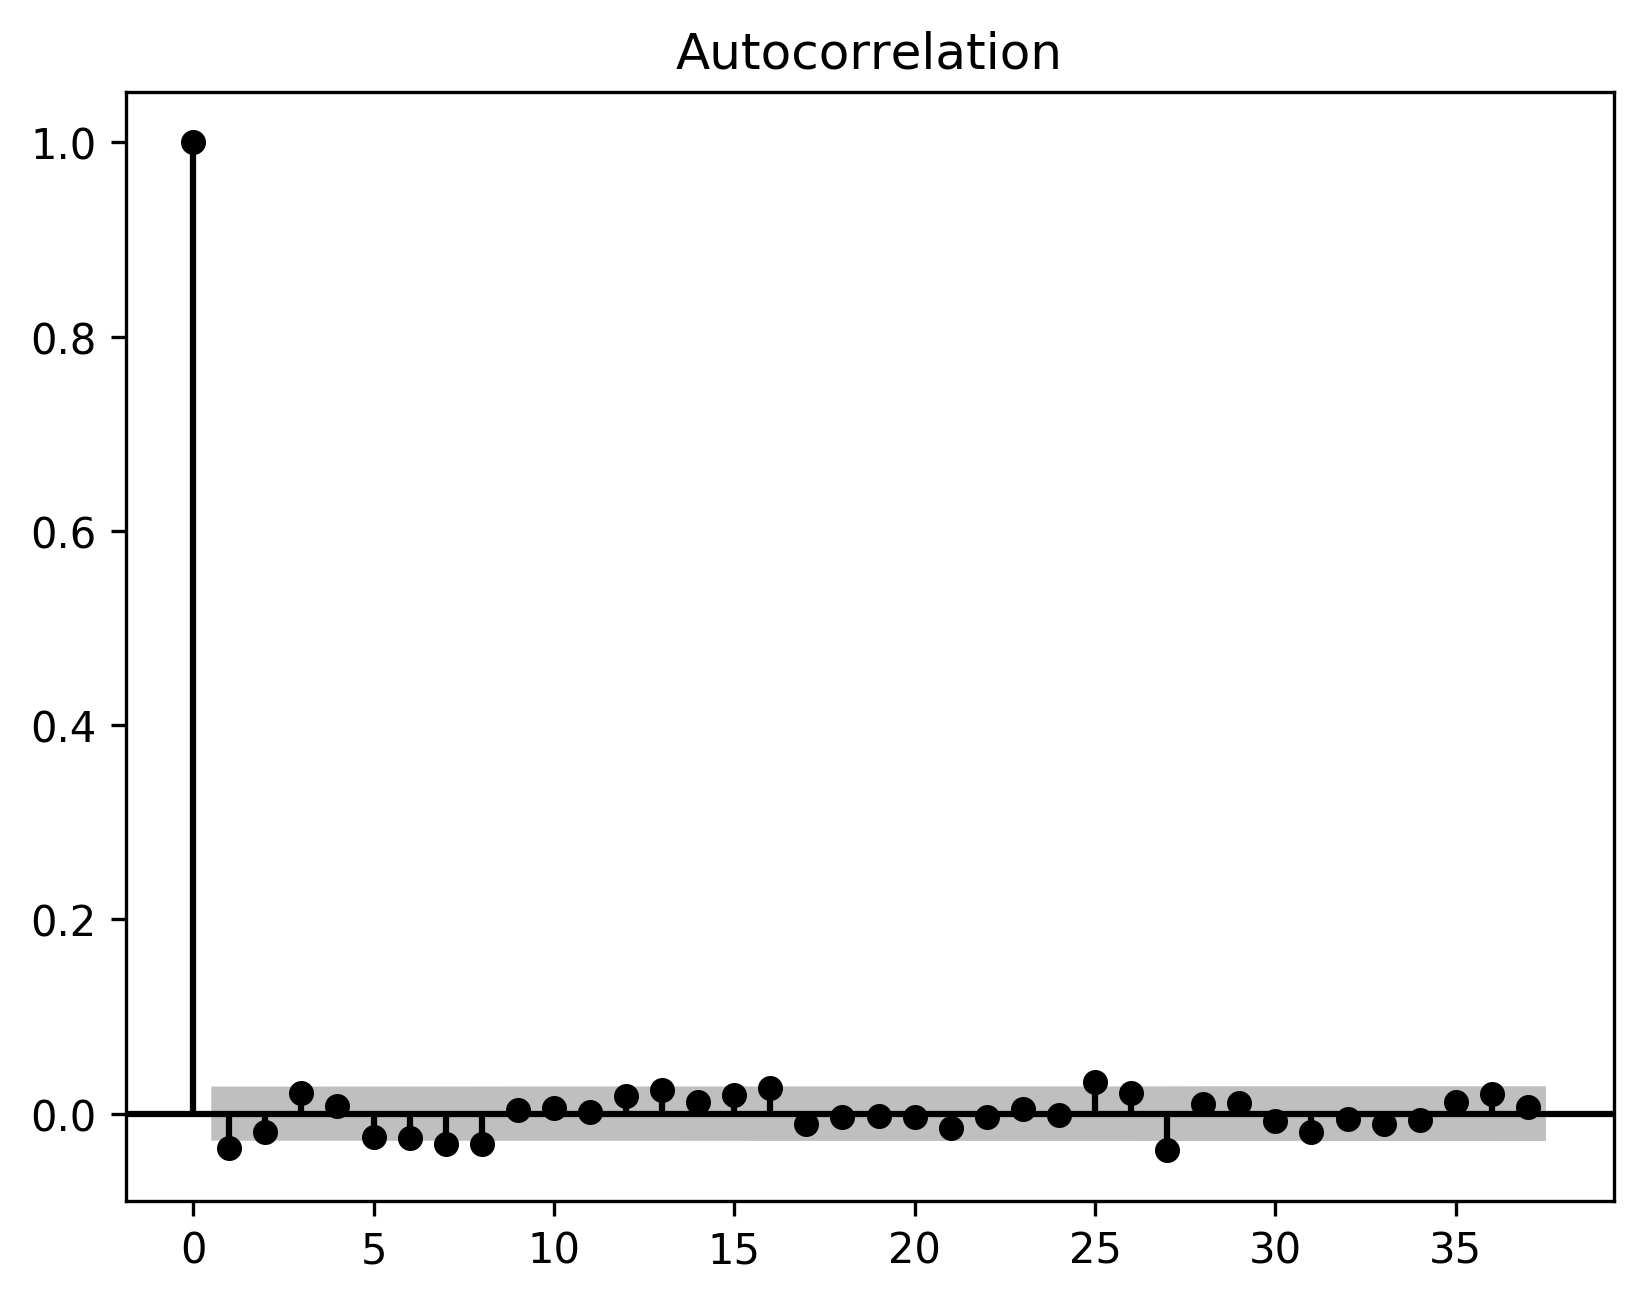
\includegraphics[width=0.45\linewidth]{figures/wti_summary/returns_acf.png}
		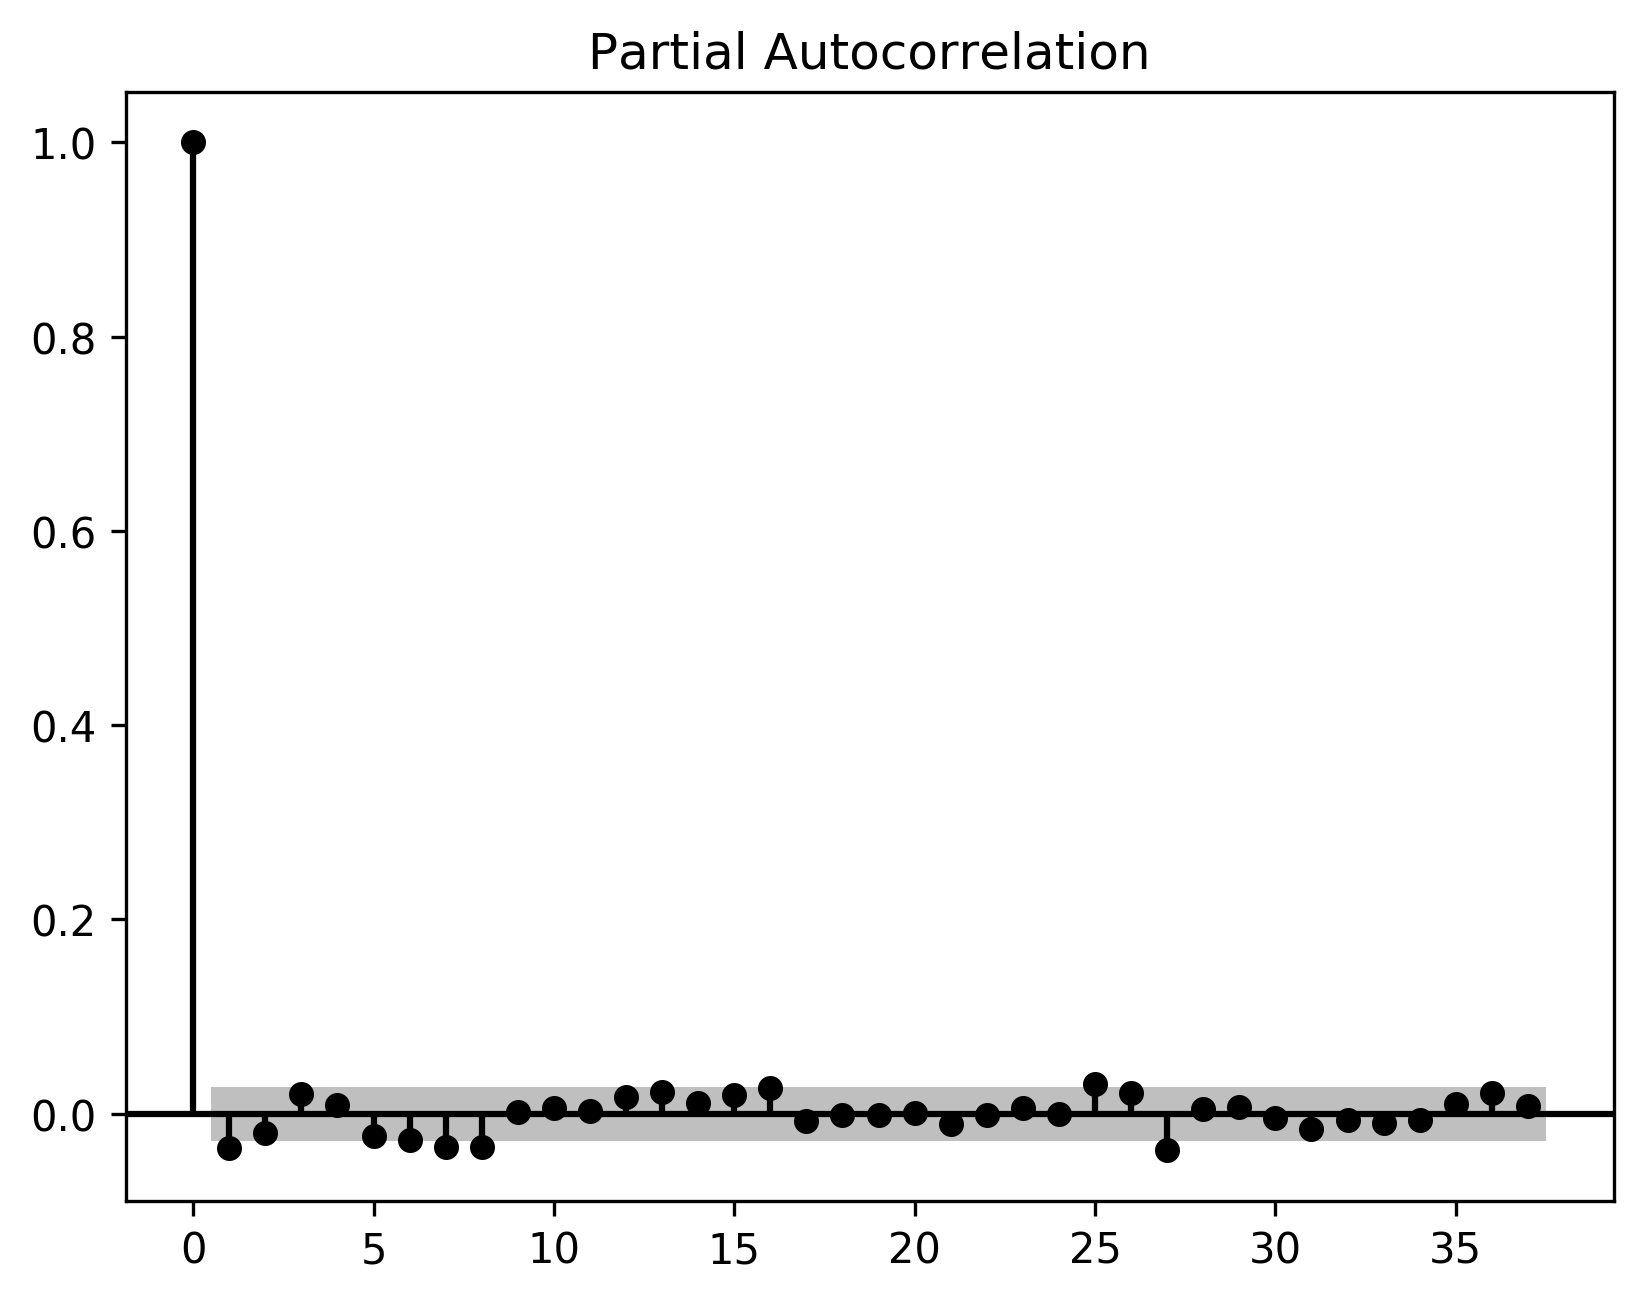
\includegraphics[width=0.45\linewidth]{figures/wti_summary/returns_pacf.png}
		\caption{ACF and PACF for Crude Oil Returns (January 2000 to September 2019)}
	\end{figure}

	\begin{figure}[H]
		\centering
		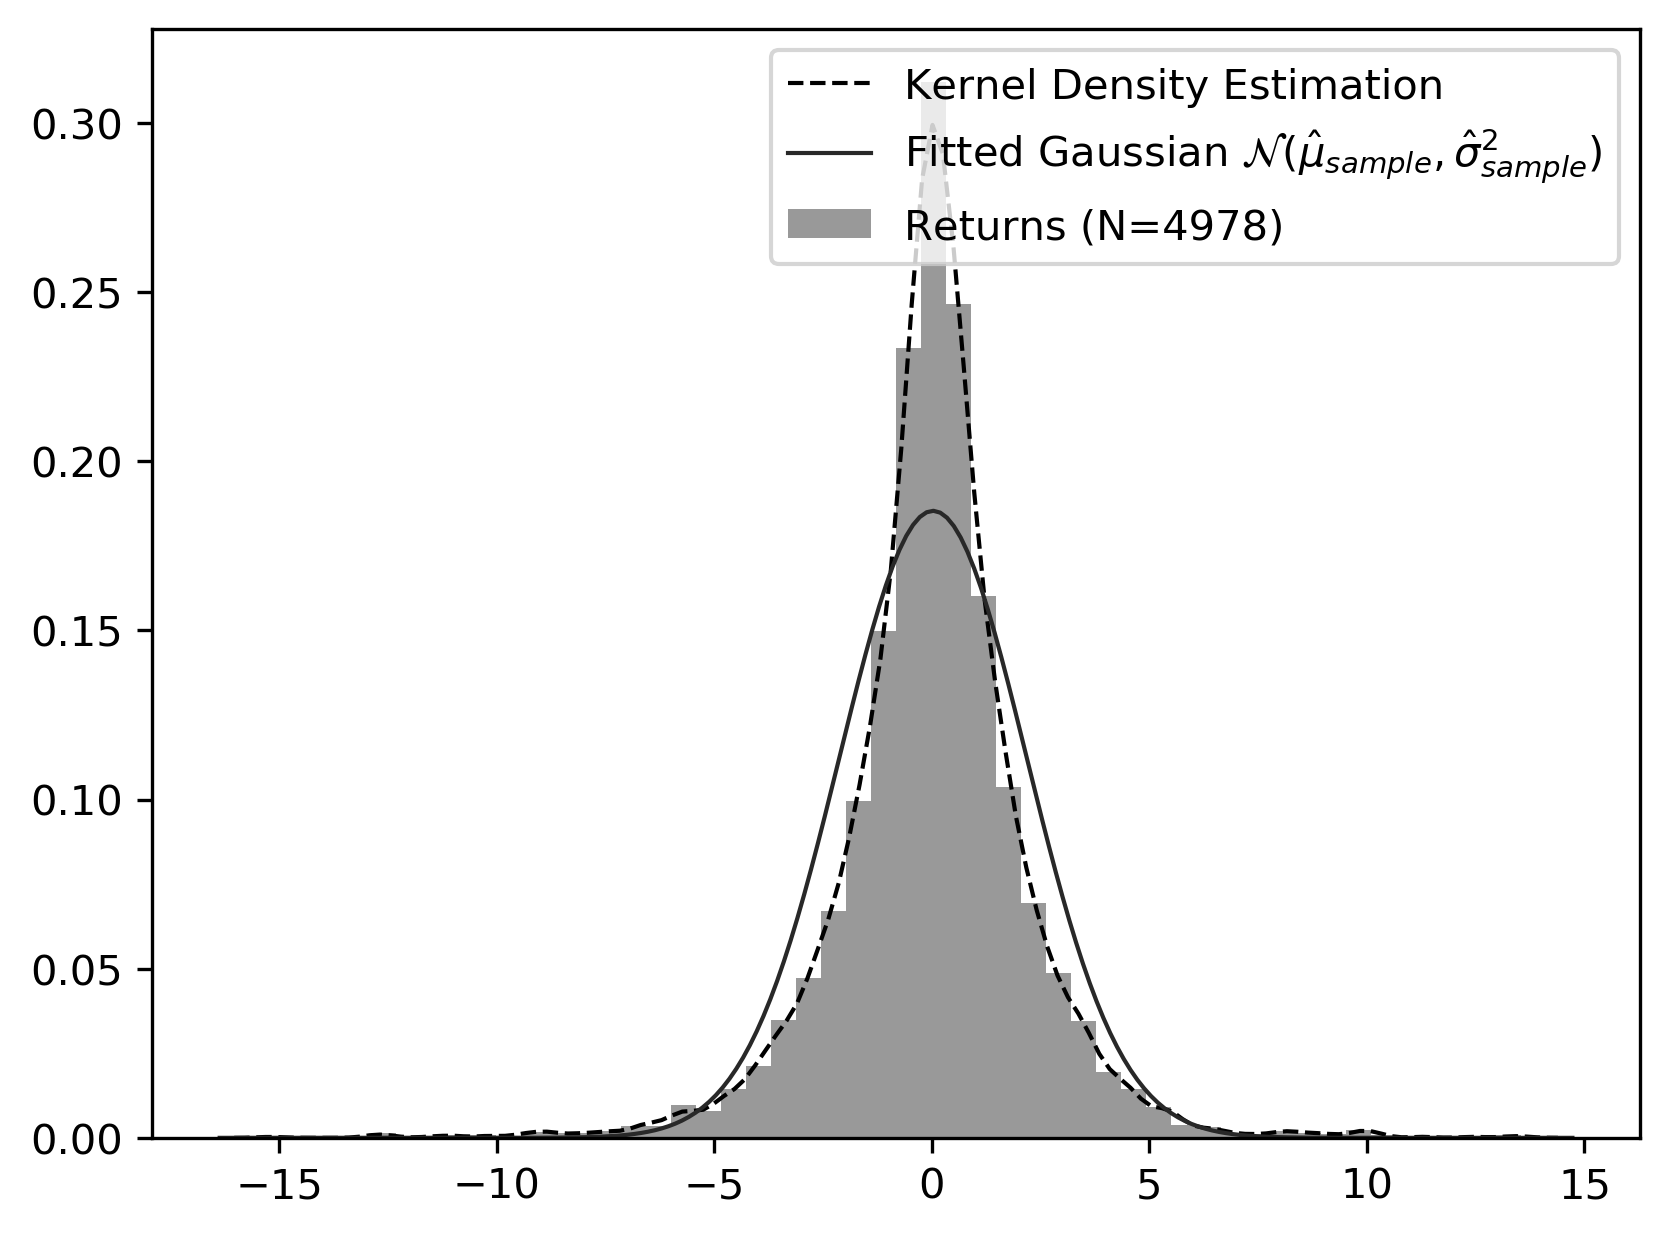
\includegraphics{figures/wti_summary/return_hist.png}
		\caption{Distribution of Crude Oil Returns (January 2000 to September 2019). The KDE line stands for the kernel density estimation for the empirical distribution. The 'Gaussian Fit' line corresponds to the density function of $\mc{N}(\hat{\mu}_\tx{sample}, \hat{\sigma}_\tx{sample})$.}
	\end{figure}

	\subsection{Missing Data in Crude Oil Dataset}
%	\paragraph{}  Given the focus of this paper is on forecasting crude oil returns, 

	\paragraph{} This paper calculates crude oil returns on one particular day $t$ by taking the difference in logged prices at $t$ and the previous trading day:
	\begin{align}
		r_t &:= \ln(p_t) - \ln(p_{t - \Delta})
	\end{align}
	where $t - \Delta$ is the last trading day before day $t$. Different gaps between consecutive trading days, $\Delta$, have salient influence on actual realized returns. Therefore, missing data issue is crucial for this paper.
	\par As mentioned before, the time gap between two observed prices are not equal. For instance, the return on a Monday can be computed by taking difference between the log close price on Monday and the previous Friday, if available. In this case, $\Delta = 3$. If the previous Friday was a holiday without valid price data, $r_t$ will be $\ln(p_\tx{Mon}) - \ln(p_{\tx{Prev Thu}})$, and $\Delta = 4$. According to \textbf{the table below}, 33 days are in this case.
	\begin{table}[H]
		\centering
		\small
		\begin{tabular}{l|c c c c c c c}
			\toprule
			Day of the week & Num. Days. & Num. Trading Days & $\Delta$=1 & 2 & 3 & 4 & 5 \\
			\midrule
			Monday & 1031 & 927 & 0 & 0 & 883 & 33 & 11 \\
			Tuesday & 1030 & 1018 & 921 & 0 & 0 & 97 & 0 \\
			Wednesday & 1030 & 1022 & 1011 & 5 & 0 & 0 & 6 \\
			Thursday & 1030 & 1002 & 994 & 8 & 0 & 0 & 0 \\
			Friday & 1030 & 986 & 969 & 17 & 0 & 0 & 0 \\
			Saturday & 1030 & 0 & 0 & 0 & 0 & 0 & 0 \\
			Sunday & 1030 & 0 & 0 & 0 & 0 & 0 & 0 \\
			\midrule
			Total & 7211 & 4955 & 3895 & 30 & 883 & 130 & 17 \\
			\bottomrule
		\end{tabular}
		\caption{The values of $\Delta$ used to calculate returns. This table only include trading days, but the first day with price observation in this dataset was dropped because it did not have a previous trading day, so return on this day cannot by computed using our definition.}
	\end{table}
	\par As mentioned before, the oil price dataset does not have any prices over weekends. \textbf{The table below} reports dates that are most frequently associated with a missing data over the span of 20 years. The pool of days with missing data is pretty consistent overtime, the market is always closed on January 1, July 4 (Independence Day) and December 25 (Christmas). The group of dates in late November are responsible for missing data on Thanksgiving holiday.
	\begin{table}[H]
		\small
		\centering
		\begin{tabular}{l|c c}
			\toprule
			Date & Counts (all) & Counts (excl. weekends) \\
			\midrule
			July 4 & 20 & 16 \\
			January 1 & 20 & 14 \\
			December 25 & 19 & 14 \\
			July 3 & 10 & 5 \\
			November 23 & 10 & 5 \\
			November 24 & 10 & 4\\
			November 25 & 10 & 3\\
			November 22 & 9 & 4 \\
			November 26 & 9 & 3 \\
			\bottomrule
		\end{tabular}
		\caption{Dates most frequently associates with missing data. Data on January 1, July 4, and December 25 are missing ever year. Because the entire dataset ranges from January 3, 2000 to September 30, 2019, missing data problems on December 25 are only reported 19 times.}
	\end{table}
 
	\subsection{Day of the Week Effect in Crude Oil Dataset}
	\subsubsection{Difference in Returns across the Week}
	\paragraph{} Gibbons and Hess' work examined returns on stocks from S\&P 500, Dow Jones 30, and Treasury Bills. They found strong negative mean returns on Monday compared with other weekdays.
	The seasonality persisted even after taking market adjustment measures, such as using mean-adjusted returns instead \cite{Hess1981}. 
	Analysis in my paper unveils a similar daily seasonality presents in crude oil returns as well.
	\textbf{Panels in the figure below} demonstrate the empirical distributions of returns on each day of the week. We can see that Mondays and Wednesdays have relatively larger variances, which again matches Gibbons and Hess' observations.
	\begin{figure}[H]
		\centering
		\small
		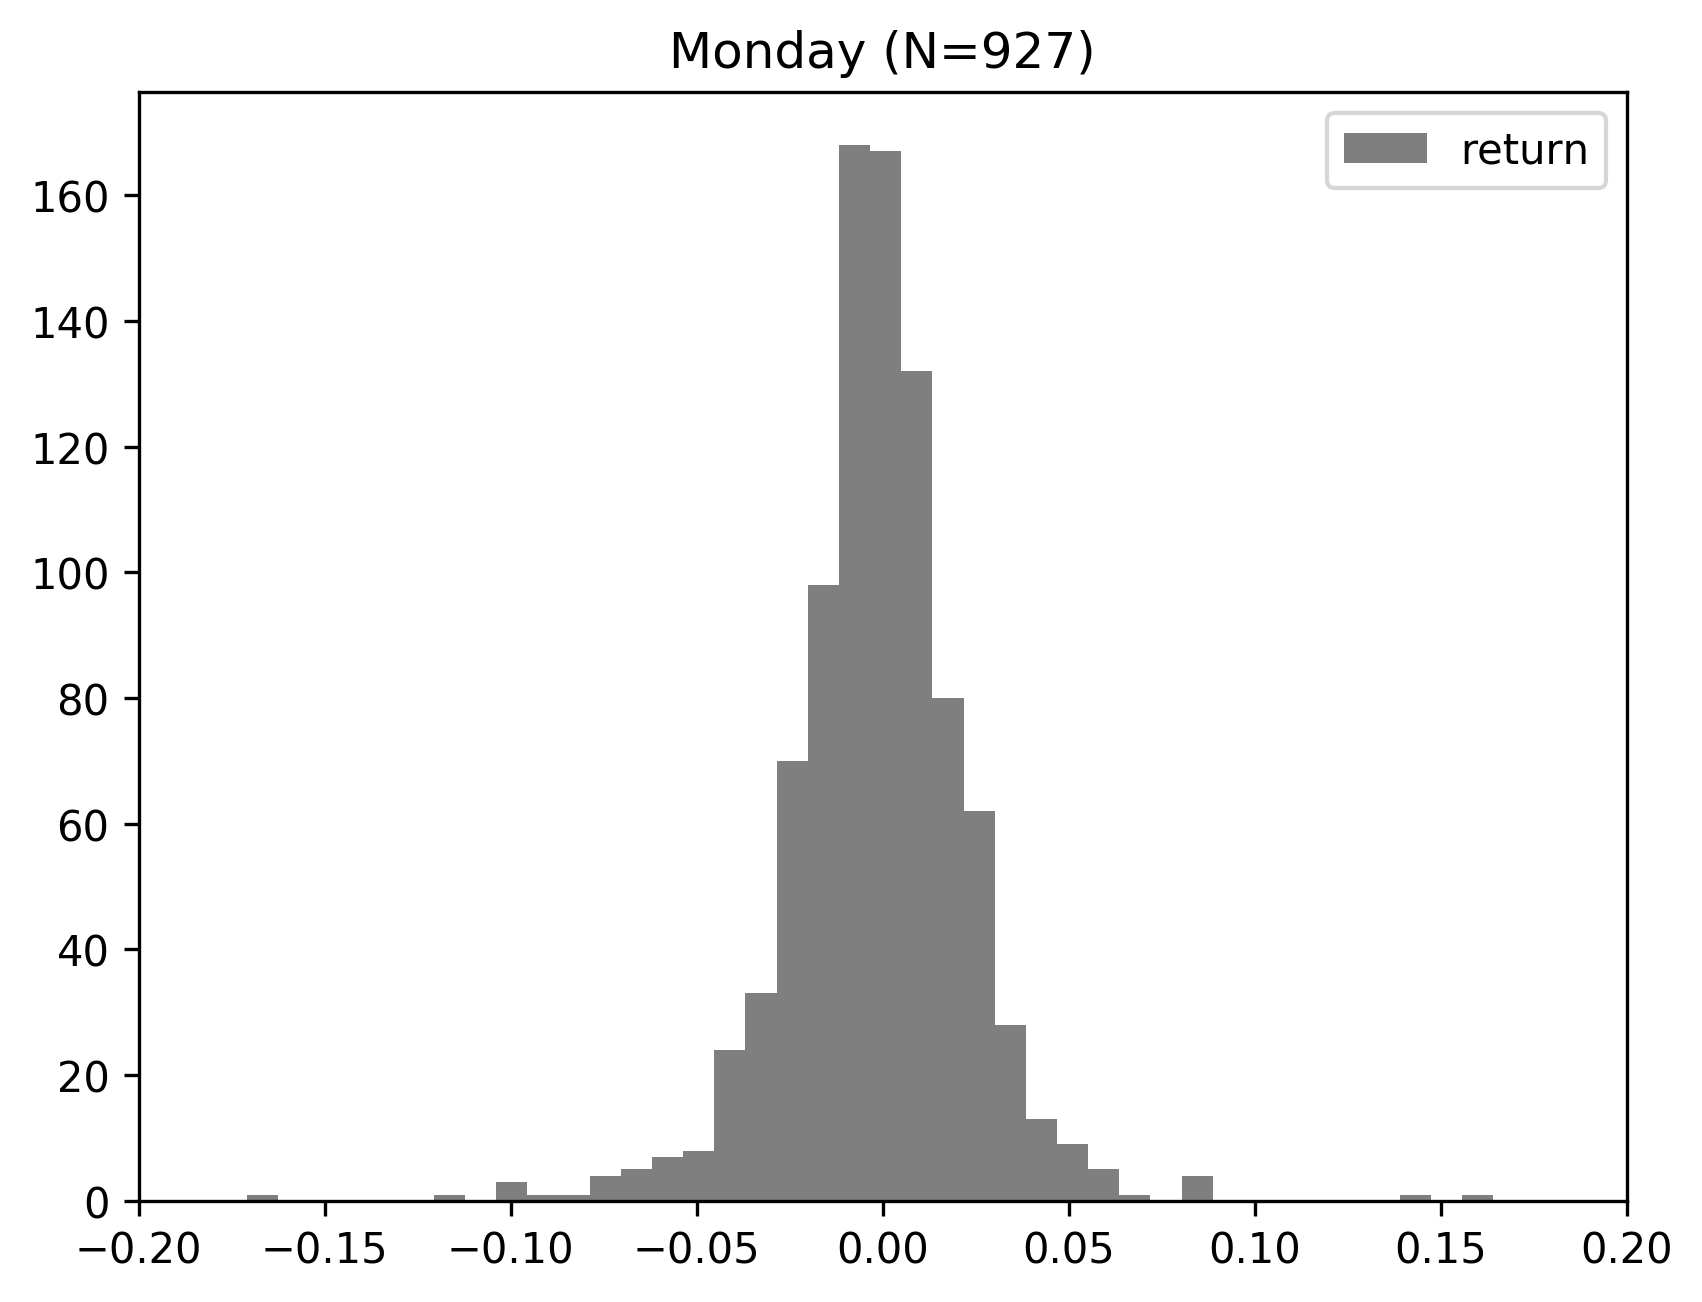
\includegraphics[width=0.45\linewidth]{figures/day_of_week_effect/dist_returns_Monday.png}
		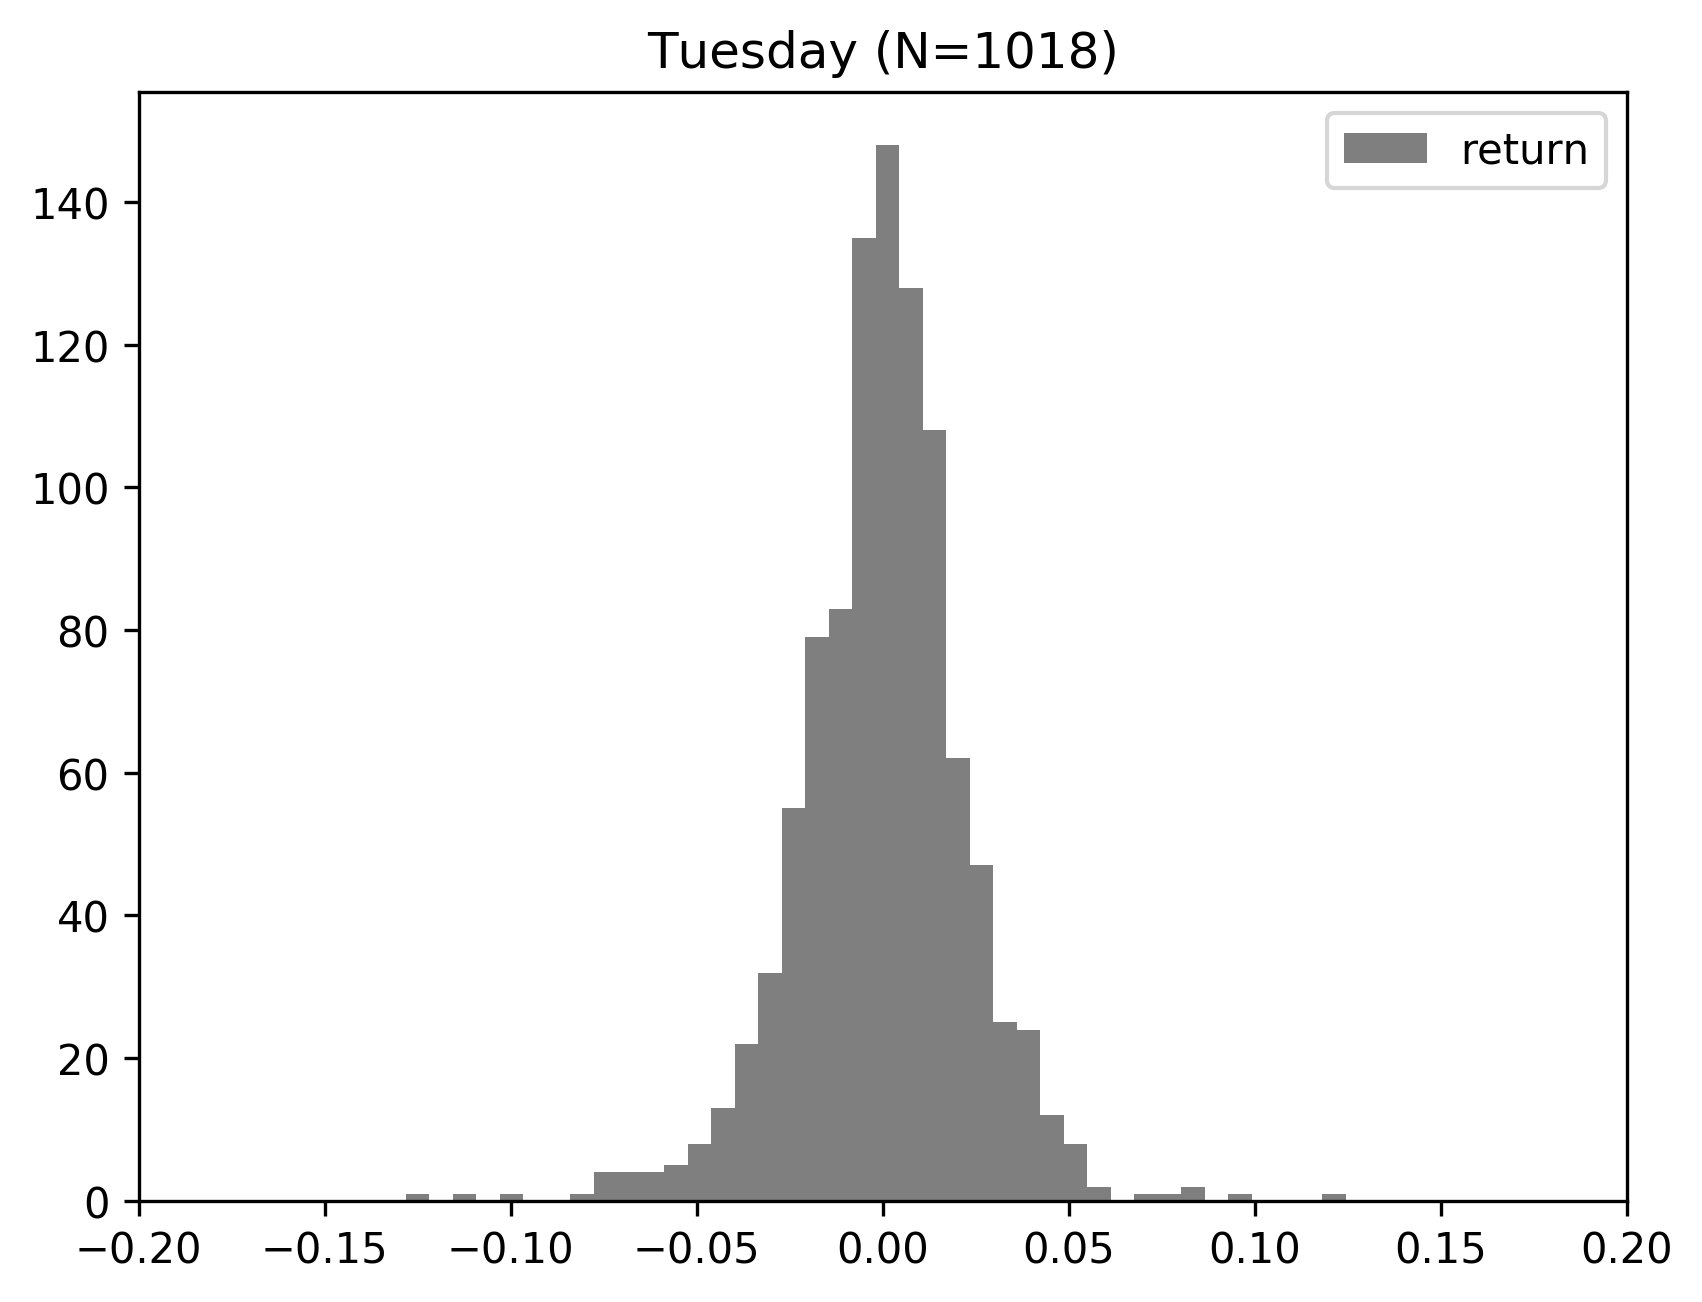
\includegraphics[width=0.45\linewidth]{figures/day_of_week_effect/dist_returns_Tuesday.png}
		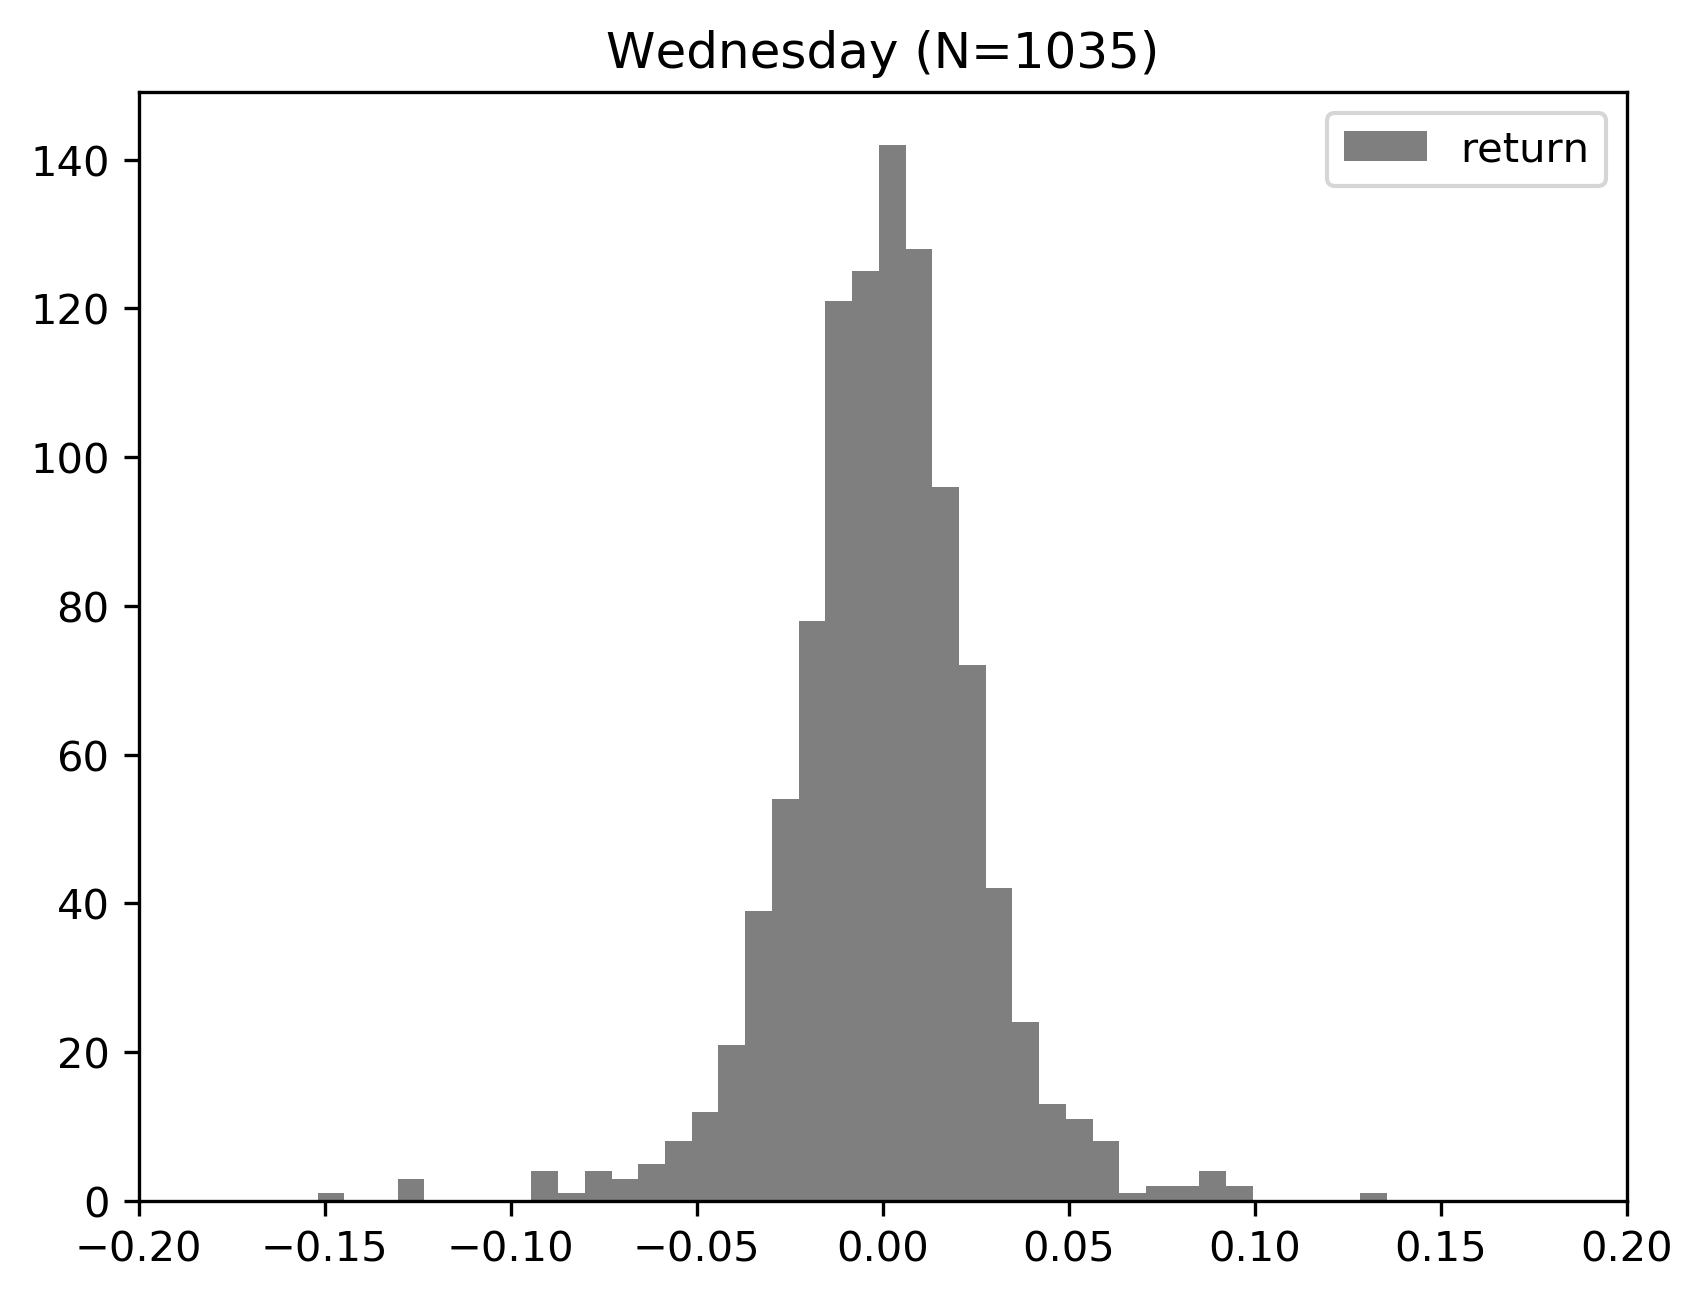
\includegraphics[width=0.45\linewidth]{figures/day_of_week_effect/dist_returns_Wednesday.png}
		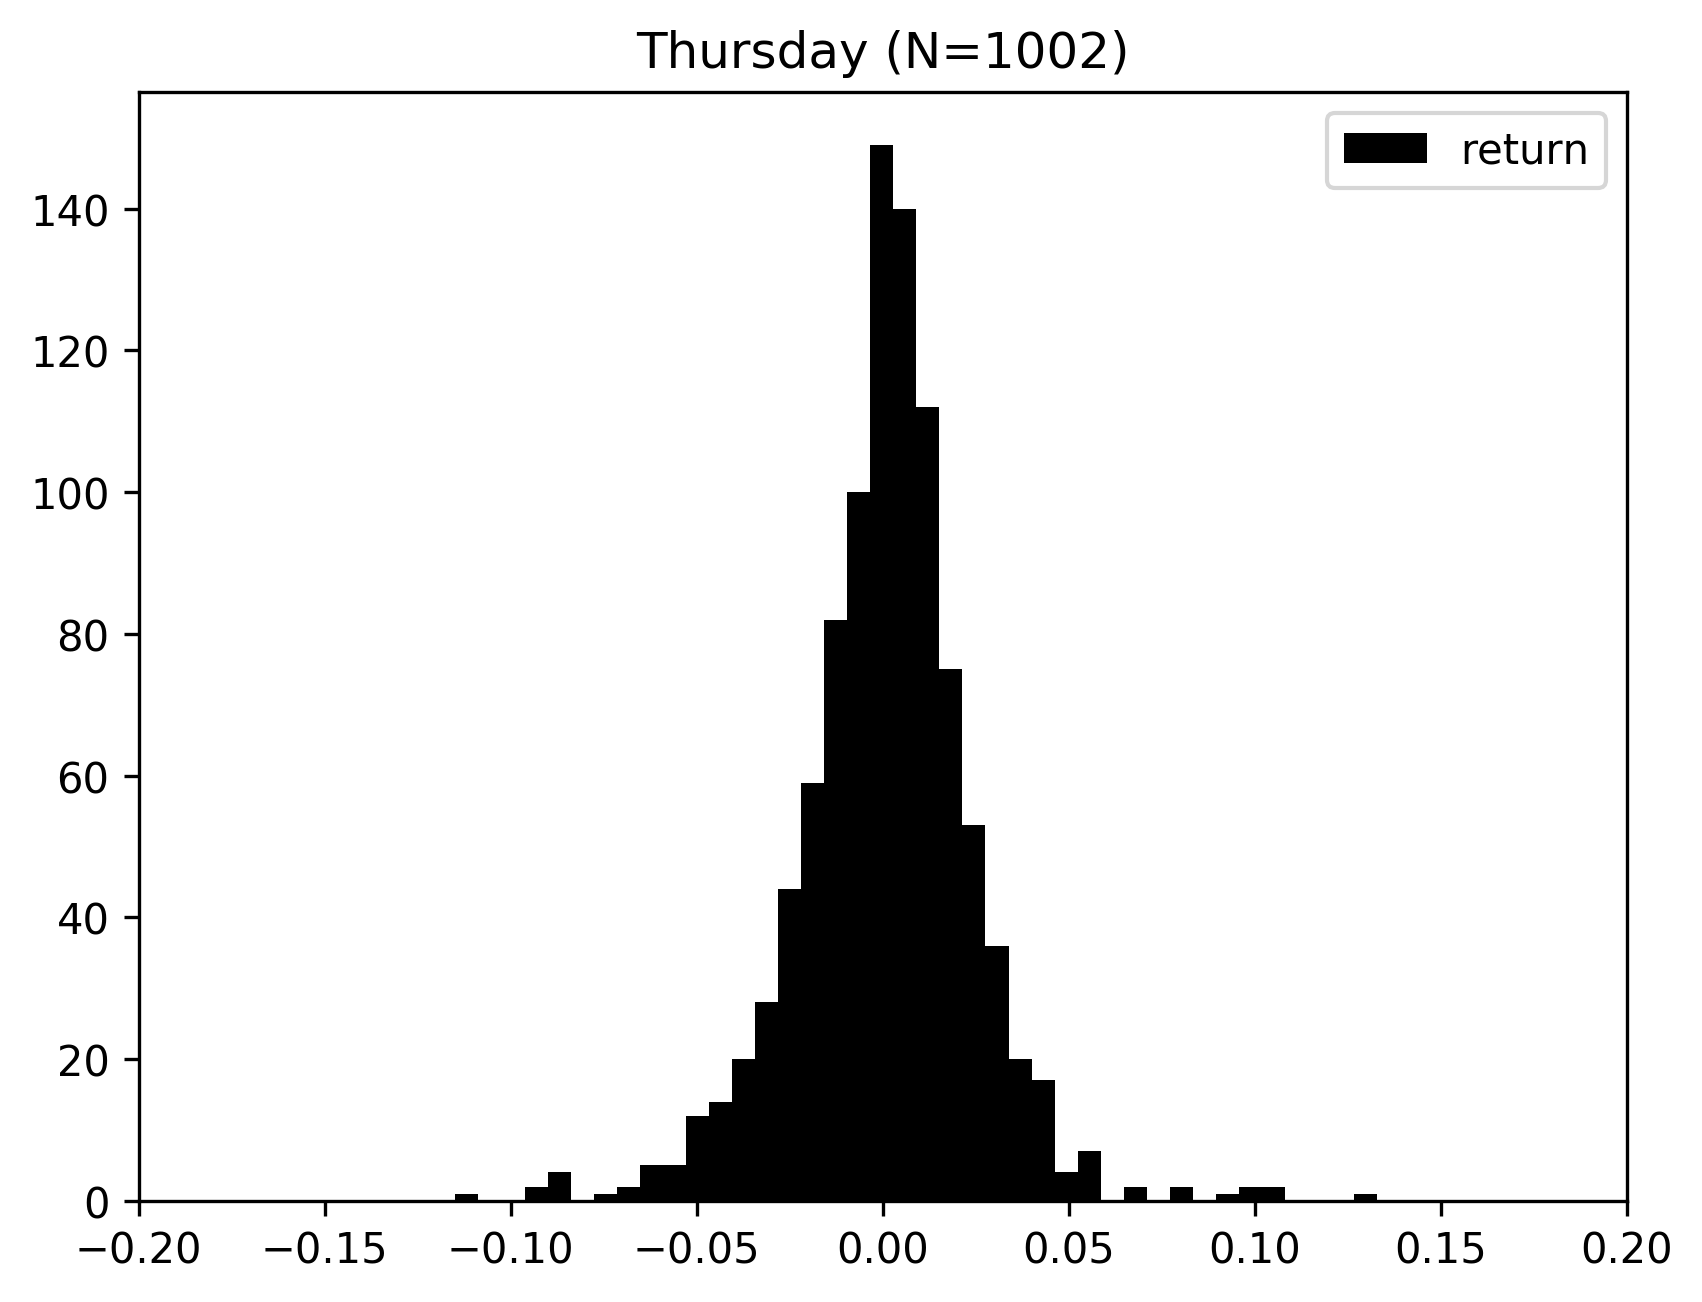
\includegraphics[width=0.45\linewidth]{figures/day_of_week_effect/dist_returns_Thursday.png}
		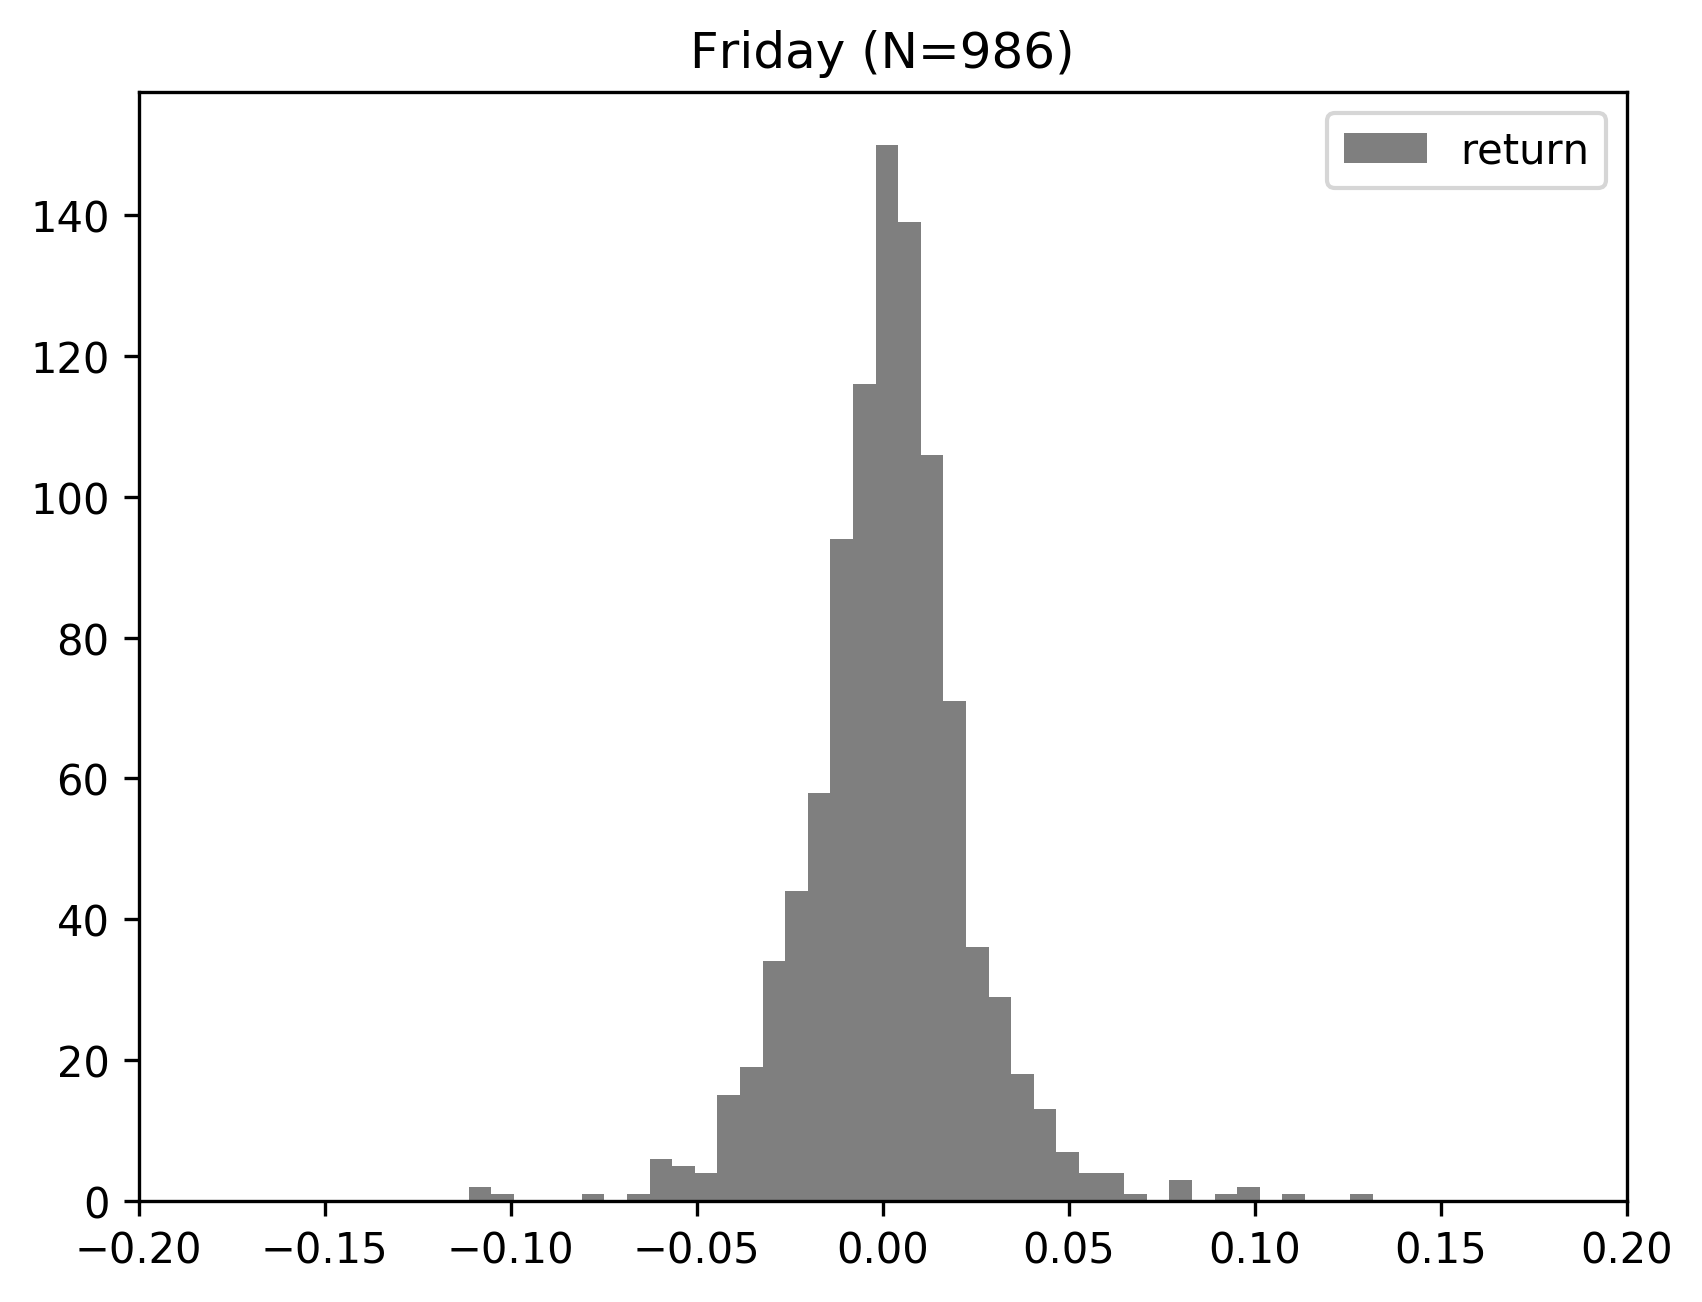
\includegraphics[width=0.45\linewidth]{figures/day_of_week_effect/dist_returns_Friday.png}
		\caption{Crude oil returns on each weekday. Weekend data are not available in the daily dataset provided by U.S. Energy Information Administration (EIA). $N$s within parentheses in figure titles denote the number of observations. See appendix for distributions of crude oil prices.}
	\end{figure}

	\par The \textbf{two tables} below provide summary statistics for prices and returns on each day. It turns out that Monday is the only weekday with a mean return significantly less than zero.
	\begin{table}[H]
		\small
		\centering
		\begin{tabular}{l|c c c c}
			\toprule
			Day of the week & Num. Obs. & Mean & Std. & $3^{rd}$ Moment \\
			\midrule
			Monday & 927 & 62.072 & 26.493 & 7081.163 \\
			Tuesday & 1019 & 61.828 & 26.317 & 6895.638 \\
			Wednesday & 1022 & 61.810 & 26.398 & 7049.810 \\
			Thursday & 1002 & 62.005 & 26.431 & 6955.555 \\
			Friday & 986 & 62.079 & 26.247 & 6676.566 \\
			\midrule
			Total & 4956 & & & \\
			\bottomrule
		\end{tabular}
		\caption{Summary statistics of crude oil prices on each day of week}
	\end{table}

	\begin{table}[H]
		\small
		\centering
		\begin{tabular}{l|c c c c}
			\toprule
			Day of the week & Num. Obs. & Mean ($P$-Value) & Std. & $3^{rd}$ Moment \\
			\midrule
			Monday & 927 & \textbf{-0.002 (0.049)} & 0.025 & -0.0000019 \\
			Tuesday & 1018 & -0.000 (0.900) & 0.023 & -0.0000031 \\
			Wednesday & 1022 & 0.000 (0.884) & 0.027 & -0.0000054 \\
			Thursday & 1002 & 0.001 (0.361) & 0.024 & -0.0000006 \\
			Friday & 986 & \textbf{0.002 (0.0311)} & 0.023 & 0.0000021 \\
			\midrule
			Total & 4955 & & & \\
			\bottomrule
		\end{tabular}
		\caption{Summary statistics of crude oil returns on each day of week. The first day (January 1, 2000) of the oil price dataset was Saturday, and the observation on the following Monday (January 3) was missing. Hence, the return on Tuesday (January 4) could not be computed because it was the first trading day in this dataset, and there are only 1018 Tuesdays in the dataset of returns. A value of $-0.000$ indicates a negative value with magnitude less than $0.0005$. $P$-values are calculated in a two-tailed $t$-test with $\mu_0 = 0$. Bold fonts indicate statistically significance at level $\alpha=0.05$.}
	\end{table}
	
	\subsubsection{Kolmogorov-Smirnov test for Distributional Similarities}
	\par Smirnov developed a non-parametric method of testing the equality between two continuous distributions, with CDFs $F(x)$ and $G(x)$ respectively, \cite{Smirnov1939}. Refer to Hodges' work for a detailed review on the Kolmogorov-Smirnov test \cite{Hodges1957}. I am using the two-tailed version of Kolmogorov-Smirnov test to check whether distributions of two different days are similar.
	Given two datasets, take returns on Mondays and Tuesdays for example, the null hypothesis says those two datasets are drawn from the same distribution, and the alternative says they are from different distributions \footnote{Different alternative hypotheses can be used in Kolmogorov–Smirnov test: i) $H_1: F(x) \geq G(x)$, ii) $H_1: F(x) \leq G(x)$, and iii) $H_1: F(x) \neq G(x)$. This paper is using the third (two-tailed) alternative hypothesis.}.
	Firstly, the Kolmogorov–Smirnov test constructs the empirical CDFs $F_{Mon, 927}(x)$ and $F_{Tue, 1018}(x)$ from the dataset. Then, the Kolmogorov–Smirnov statistic measures the maximum discrepancy between two distribution functions, which is
	\begin{align}
		D := \sup_x \abs{F_{Mon, 927}(x) - F_{Tue, 1018}(x)} \in [0, 1]
	\end{align}
	A smaller $D$-statistic implies stronger distributional similarity between two distributions. For instance, when $F_{Mon, 927}(x)$ and $F_{Tue, 1018}(x)$ are exactly the same, the $D$-statistic is zero. In contrast, let $X=0$ and $Y=1$ be two deterministic random variables, in this case, $D_{X, Y} = 1$.\\
	The test rejects $H_0$ at a significance level of $\alpha$ if 
	\begin{align}
		D > \sqrt{-\frac{1}{2} \ln \frac{\alpha}{2}} \sqrt{\frac{n+m}{nm}}
	\end{align}
	where $m$ and $n$ denote sizes of two datasets.
	\begin{table}[H]
		\small
		\centering
		\begin{tabular}{l|c|c|c|c|c}
			\toprule
			$D$-Statistic ($P$-Value)& Monday & Tuesday & Wednesday & Thursday & Friday \\
			\midrule
			Monday    & 0.000 (1.000) & \textbf{0.061 (0.048)} & \textbf{0.065 (0.030)} & \textbf{0.092 (0.001)} & \textbf{0.092 (0.001)} \\
			Tuesday   &               & 0.000 (1.000) & \textbf{0.044 (0.260)} & 0.036 (0.505) & 0.044 (0.264) \\
			Wednesday &               &               & 0.000 (1.000) & 0.053 (0.114) & \textbf{0.073 (0.009)} \\
			Thursday  &               &               &               & 0.000 (1.000) & 0.025 (0.900) \\
			Friday    &               &               &               &               & 0.000 (1.000) \\
			\bottomrule
		\end{tabular}
		\caption{The Kolmogorov-Smirnov $D$-Statistic for all pairs of distributions. Bold font indicates the null hypothesis is rejected at a significance level of 0.05, which implies discrepancy in distributions.}
	\end{table}
	\textbf{The table above} presents the Kolmogorov-Smirnov $D$-Statistic for distributions of every pairs of days. At a significance level of 0.05, we can see that Mondays follow a distribution significantly different from distributions of other weekdays follow. Because the dataset does not contain weekend data, returns on Mondays is always computed using the difference between log prices on Monday and the previous Friday (Thursday if Friday is not a trading day and so on). Therefore, returns associated with Mondays pick the weekend effect. In fact, the distribution of returns on Mondays (over weekends) is the only one with negative mean among distributions of all five days.

	\subsection{News and Sentiment Datasets}
	\paragraph{} The event sentiment dataset from RavenPack News Analytics (RPNA) tracks and analyzes all information of companies, organizations, countries, commodities, and currencies from four major sources: Dow Jones Newswires, Wall Street Journal, Barron’s and MarketWatch.
	\par The dataset covers events from January 1, 2000, to September 30, 2019. RavenPack records the exact date and coordinated universal time (UTC) when each news is published.s
	\par For each piece of news, the dataset links it to a unique entity name attribute. To filter out noise data less relevant to crude oil returns, this paper selects the subset of news with crude oil topic. There are 106, 960 entries from the original dataset left, lead to 15 events per day on average. In the figure below, panel A presents a distribution of ESS for all news related to crude oil in the time span of 20 years and panel B shows all distributions of events within each year.

	\par Moreover, the dataset categorizes each event following the RavenPack taxonomy.
	\begin{figure}[H]
		\centering
		\small
		\begin{enumerate}[(i)]
			\item topic;
			\item group;
			\item type;
			\item sub-type;
			\item property;
			\item category: fine details.
		\end{enumerate}
		\caption{Ravenpack taxonomy \todo{Add examples of each level.} \todo{Add definitions of each level.}}
	\end{figure}
	\par To proxy the potential economic impact upon news arrival and afterwards, Ravenpack assigns each piece of news an Event Sentiment Score (ESS) between 0 and 100 using an algorithm combines results from surveying financial experts and pattern matching. An ESS of 100 indicates extreme positive short-term positive financial or economic impact. In contrast, a 0 ESS score indicates extreme negative impact. And a ESS of 50 indicates exact neutral news. From this point, scores are normalized by subtracting 50, so that the sign of normalized ESS matches the nature of news, and a zero score represents a neutral news. \textbf{The histogram below} plots the distribution of normalized ESS for all news about crude oil. It turns out that only a small portion of news is purely neutral (i.e., with zero ESS)
	\todo{(Probably move this part to the 'classification' section.)}
	\begin{figure}[H]
		\centering
		\small
		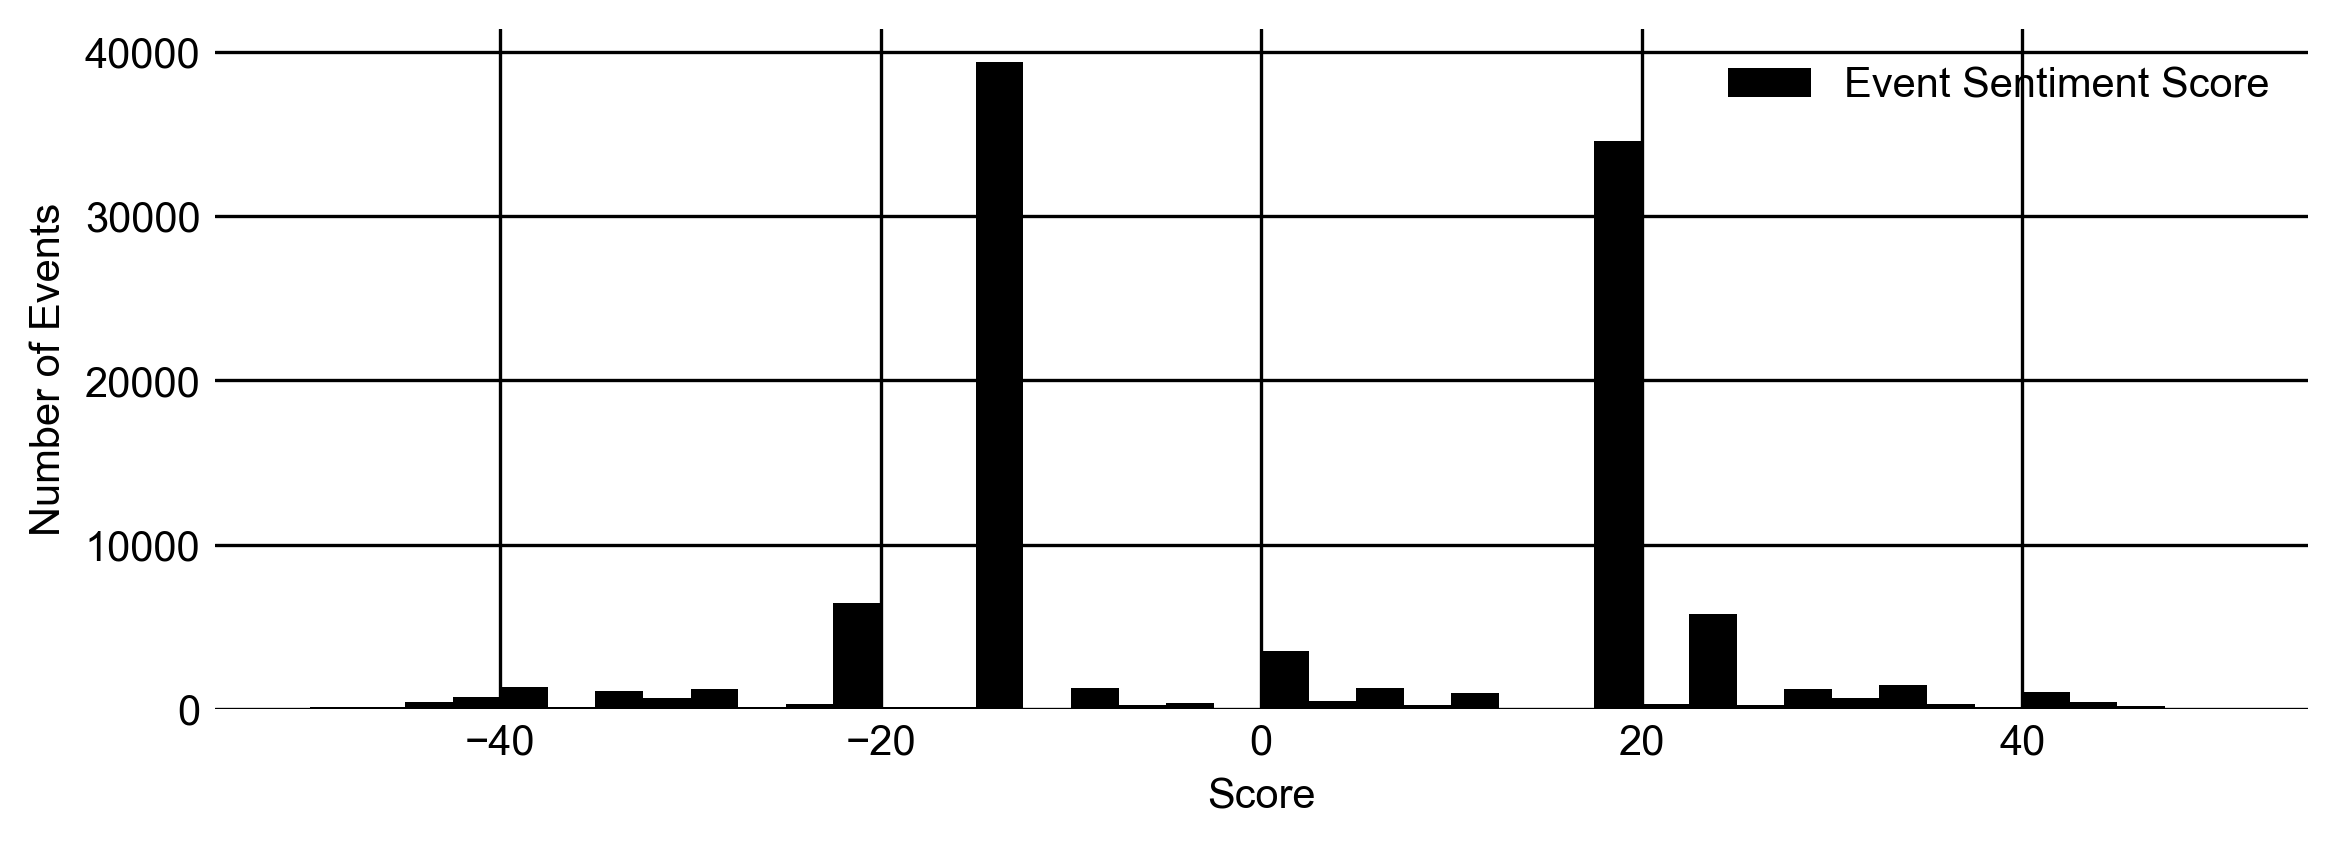
\includegraphics[width=\linewidth]{figures/event_classification/hist_ess_all.png}
		\caption{Distribution of Event Sentiment Scores of all 106,960 news items.}
	\end{figure}

	\par It is worth mentioning that ESS measures the potential impact on the topic of this news. For example, a civil unrest in a middle east country is often considered as news forerun negative economic impact, especially for the country itself.
	However, such news is in general associated with positive ESS scores because the expected negative supply shocks carried by these news are typically positively correlated crude oil prices and returns. \textbf{Tables below} present a list of categories frequently associated with positive and negatives news. From these two table we can see that the majority of themes of positive news would impact crude oil prices and returns positively.
	\begin{table}[H]
		\centering
		\small
		\begin{tabular}{l|c}
			\toprule
			Category & Number of positive news \\
			\midrule
			commodity-price-gain & 22,893 \\
			commodity-futures-gain & 11,648 \\
			supply-decrease-commodity & 5,845 \\
			imports-up & 2,705 \\
			commodity-buy-target & 1,171 \\
			demand-increase-commodity & 1,070 \\
			exports-down & 1,020 \\
			other 28 categories & 3,014 \\
			\midrule
			all positive news & 49,366 \\
			\bottomrule
		\end{tabular}
		\caption{Most frequent categories of positive news. Only categories with frequency greater than 1,000 are shown in this table.}
	\end{table}

	\begin{table}[H]
		\centering
		\small
		\begin{tabular}{l|c}
			\toprule
			Category & Number of negative news \\
			\midrule
			commodity-price-loss & 26,475 \\
			commodity-futures-loss & 12,818 \\
			supply-increase-commodity & 6,629 \\
			imports-down & 2,017 \\
			exports-up & 1308 \\
			resource-discovery-commodity & 1,179 \\
			technical-view-bearish & 1,172 \\
			other 24 categories & 2,517 \\
			\midrule
			all negative news & 54,115 \\
			\bottomrule
		\end{tabular}
		\caption{Most frequent categories of positive news. Only categories with frequency greater than 1,000 are shown in this table.}
	\end{table}
	
	\begin{table}[H]
		\centering
		\small
		\caption{Summary Statistics for Daily News Arrival by Years}
		\begin{tabular}{l|c|c|c|c|c|c|c}
		\toprule
		Year & Mean & Median & Std. & Min & Max & $3^{rd}$ Moment & $4^{th}$ Moment \\
		\midrule
2000 & 10.990 & 10.000 & 7.883 & 1.000 & 48.000 & 624.140 & 20580.847\\
2001 & 14.929 & 14.000 & 9.225 & 1.000 & 51.000 & 489.795 & 25704.202\\
2002 & 4.807 & 4.000 & 3.452 & 1.000 & 19.000 & 60.569 & 801.811\\
2003 & 6.519 & 4.000 & 6.241 & 1.000 & 39.000 & 478.654 & 12369.937\\
2004 & 24.608 & 23.000 & 16.612 & 1.000 & 84.000 & 3190.837 & 261755.365\\
2005 & 20.921 & 21.000 & 12.480 & 1.000 & 57.000 & 668.782 & 71292.410\\
2006 & 21.375 & 21.000 & 13.224 & 1.000 & 58.000 & 311.175 & 72550.280\\
2007 & 19.695 & 18.000 & 12.724 & 1.000 & 66.000 & 1080.233 & 80582.446\\
2008 & 22.264 & 23.000 & 14.481 & 1.000 & 66.000 & 773.619 & 114575.879\\
2009 & 16.642 & 16.000 & 10.145 & 1.000 & 48.000 & 229.465 & 26102.072\\
2010 & 17.373 & 18.000 & 10.704 & 1.000 & 52.000 & 223.408 & 32208.647\\
2011 & 22.252 & 23.000 & 12.838 & 1.000 & 65.000 & 346.488 & 76634.229\\
2012 & 22.679 & 23.000 & 13.582 & 1.000 & 65.000 & 327.492 & 89356.087\\
2013 & 17.048 & 17.000 & 10.419 & 1.000 & 57.000 & 405.999 & 35381.337\\
2014 & 16.193 & 13.000 & 13.162 & 1.000 & 69.000 & 3434.647 & 167509.547\\
2015 & 22.334 & 20.000 & 14.945 & 1.000 & 80.000 & 2368.778 & 171467.903\\
2016 & 24.361 & 22.000 & 16.265 & 1.000 & 101.000 & 3602.310 & 285093.246\\
2017 & 15.428 & 14.000 & 10.105 & 1.000 & 58.000 & 815.307 & 43032.009\\
2018 & 15.692 & 15.000 & 10.870 & 1.000 & 93.000 & 1976.611 & 145822.537\\
2019 & 15.157 & 14.000 & 9.584 & 1.000 & 65.000 & 968.021 & 47684.600\\
		\bottomrule
		\end{tabular}
	\end{table}
	
	\begin{table}[H]
		\centering
		\small
		\caption{Average Numbers of News on Each Day}
		\begin{tabular}{l|c|c|c|c|c|c|c}
			\toprule
			Year & Monday &Tuesday &Wednesday &Thursday &Friday &Saturday &Sunday \\ 
			\midrule
2000 & 11.157 & 14.135 & 13.077 & 11.885 & 9.769 & 1.643 & 1.500 \\
2001 & 12.547 & 17.569 & 21.327 & 15.058 & 14.078 & 1.000 & 1.200 \\
2002 & 5.771 & 5.019 & 5.224 & 3.980 & 5.469 & 1.200 & 1.600 \\
2003 & 7.080 & 6.529 & 9.942 & 6.863 & 5.490 & 1.200 & 1.136 \\
2004 & 24.058 & 28.981 & 39.250 & 28.660 & 22.302 & 2.182 & 2.240 \\
2005 & 21.462 & 21.846 & 33.596 & 24.654 & 19.000 & 1.765 & 2.259 \\
2006 & 22.981 & 24.885 & 35.904 & 24.846 & 19.731 & 1.346 & 2.161 \\
2007 & 19.792 & 21.385 & 33.577 & 23.846 & 16.769 & 1.941 & 2.212 \\
2008 & 24.788 & 26.415 & 36.415 & 26.269 & 25.250 & 2.207 & 3.065 \\
2009 & 16.058 & 21.346 & 29.192 & 16.925 & 15.538 & 1.688 & 2.366 \\
2010 & 16.327 & 23.058 & 28.654 & 20.596 & 17.135 & 2.261 & 2.932 \\
2011 & 23.769 & 28.577 & 32.904 & 25.750 & 19.942 & 2.053 & 3.441 \\
2012 & 22.340 & 26.654 & 36.423 & 26.981 & 25.118 & 3.783 & 2.756 \\
2013 & 16.673 & 19.642 & 28.588 & 19.038 & 15.846 & 2.500 & 2.366 \\
2014 & 15.510 & 18.846 & 25.113 & 16.923 & 15.529 & 2.167 & 2.467 \\
2015 & 23.019 & 27.135 & 35.558 & 23.189 & 19.843 & 2.091 & 2.957 \\
2016 & 23.333 & 29.192 & 38.462 & 24.808 & 23.077 & 2.190 & 2.105 \\
2017 & 14.220 & 16.788 & 25.192 & 16.077 & 14.039 & 1.696 & 1.667 \\
2018 & 13.654 & 19.059 & 24.712 & 18.635 & 15.235 & 2.586 & 2.143 \\
2019 & 11.263 & 15.872 & 24.600 & 15.026 & 13.795 & 1.923 & 1.500 \\
		\bottomrule
		\end{tabular}
	\end{table}

	\subsection{Classifying News Type}
	
	\subsection{Case Studies of Events}
	\subsubsection{Positive Spike on November 30, 2016}
	\begin{figure}[H]
		\centering
		\small
		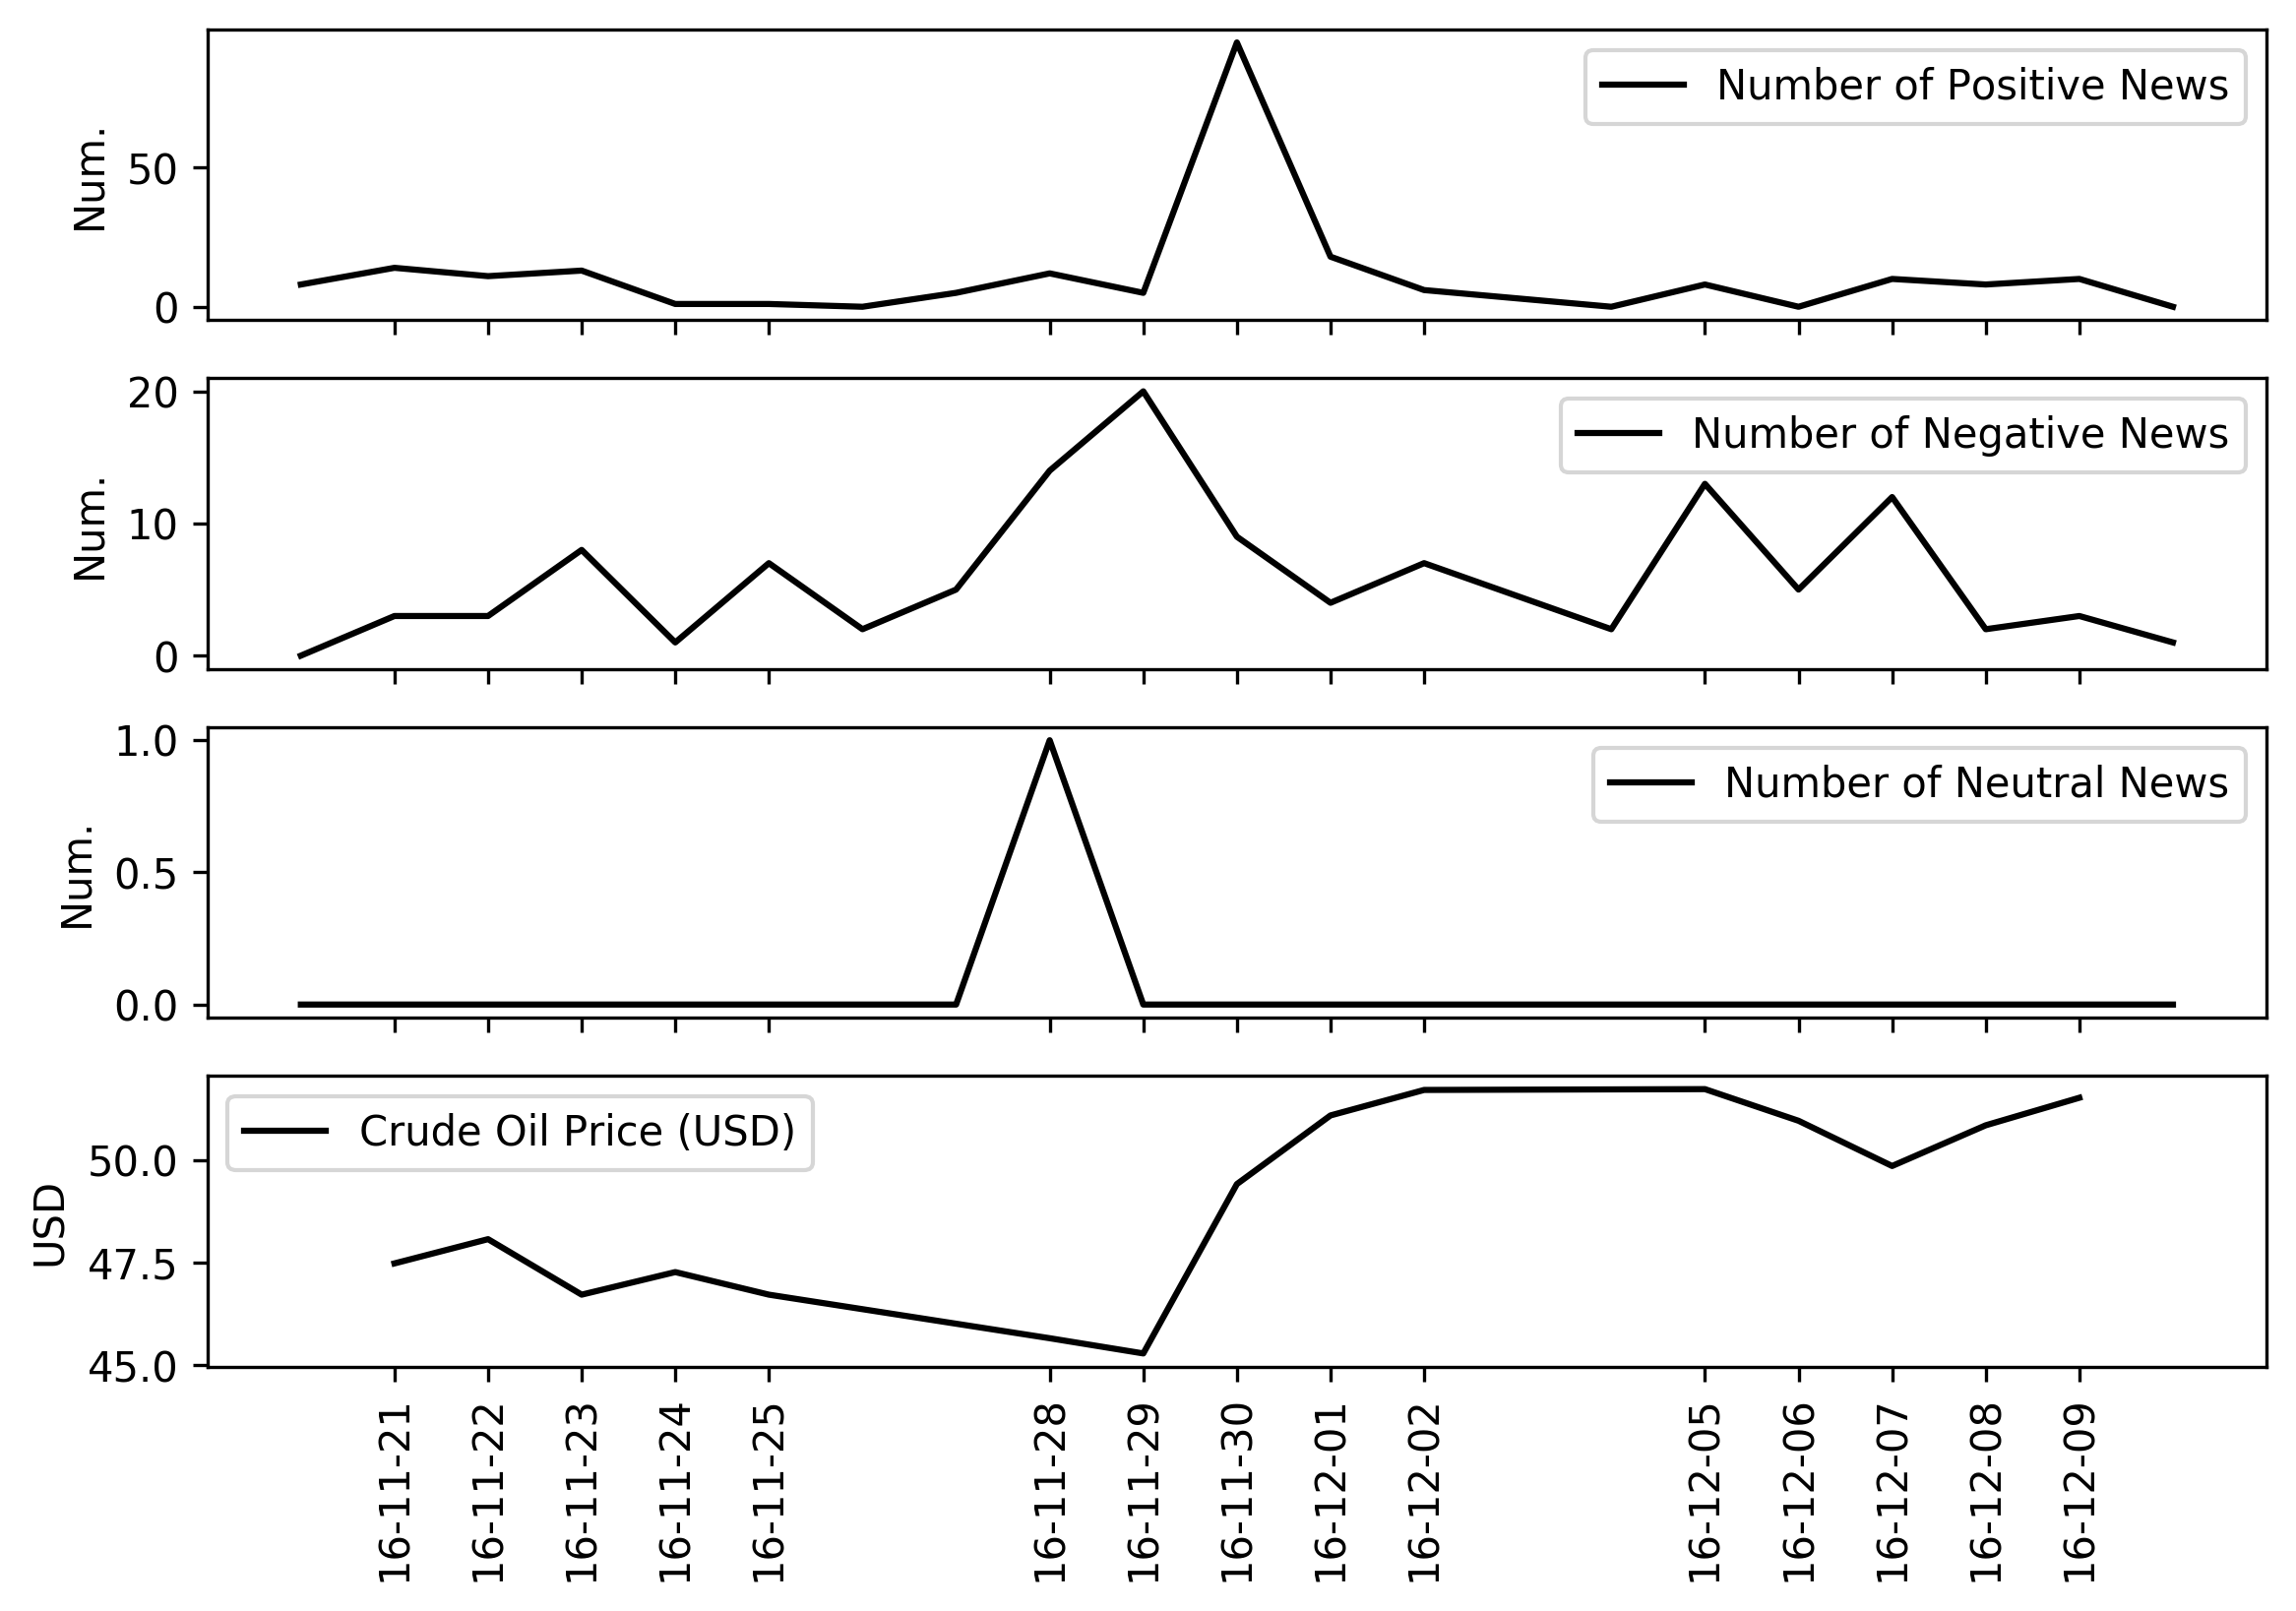
\includegraphics[width=\linewidth]{figures/case_studies/20161130_10d.png}
		\caption{}
	\end{figure}
	
	\subsubsection{Negative Spike on December 6, 2018}
	\begin{figure}[H]
		\centering
		\small
		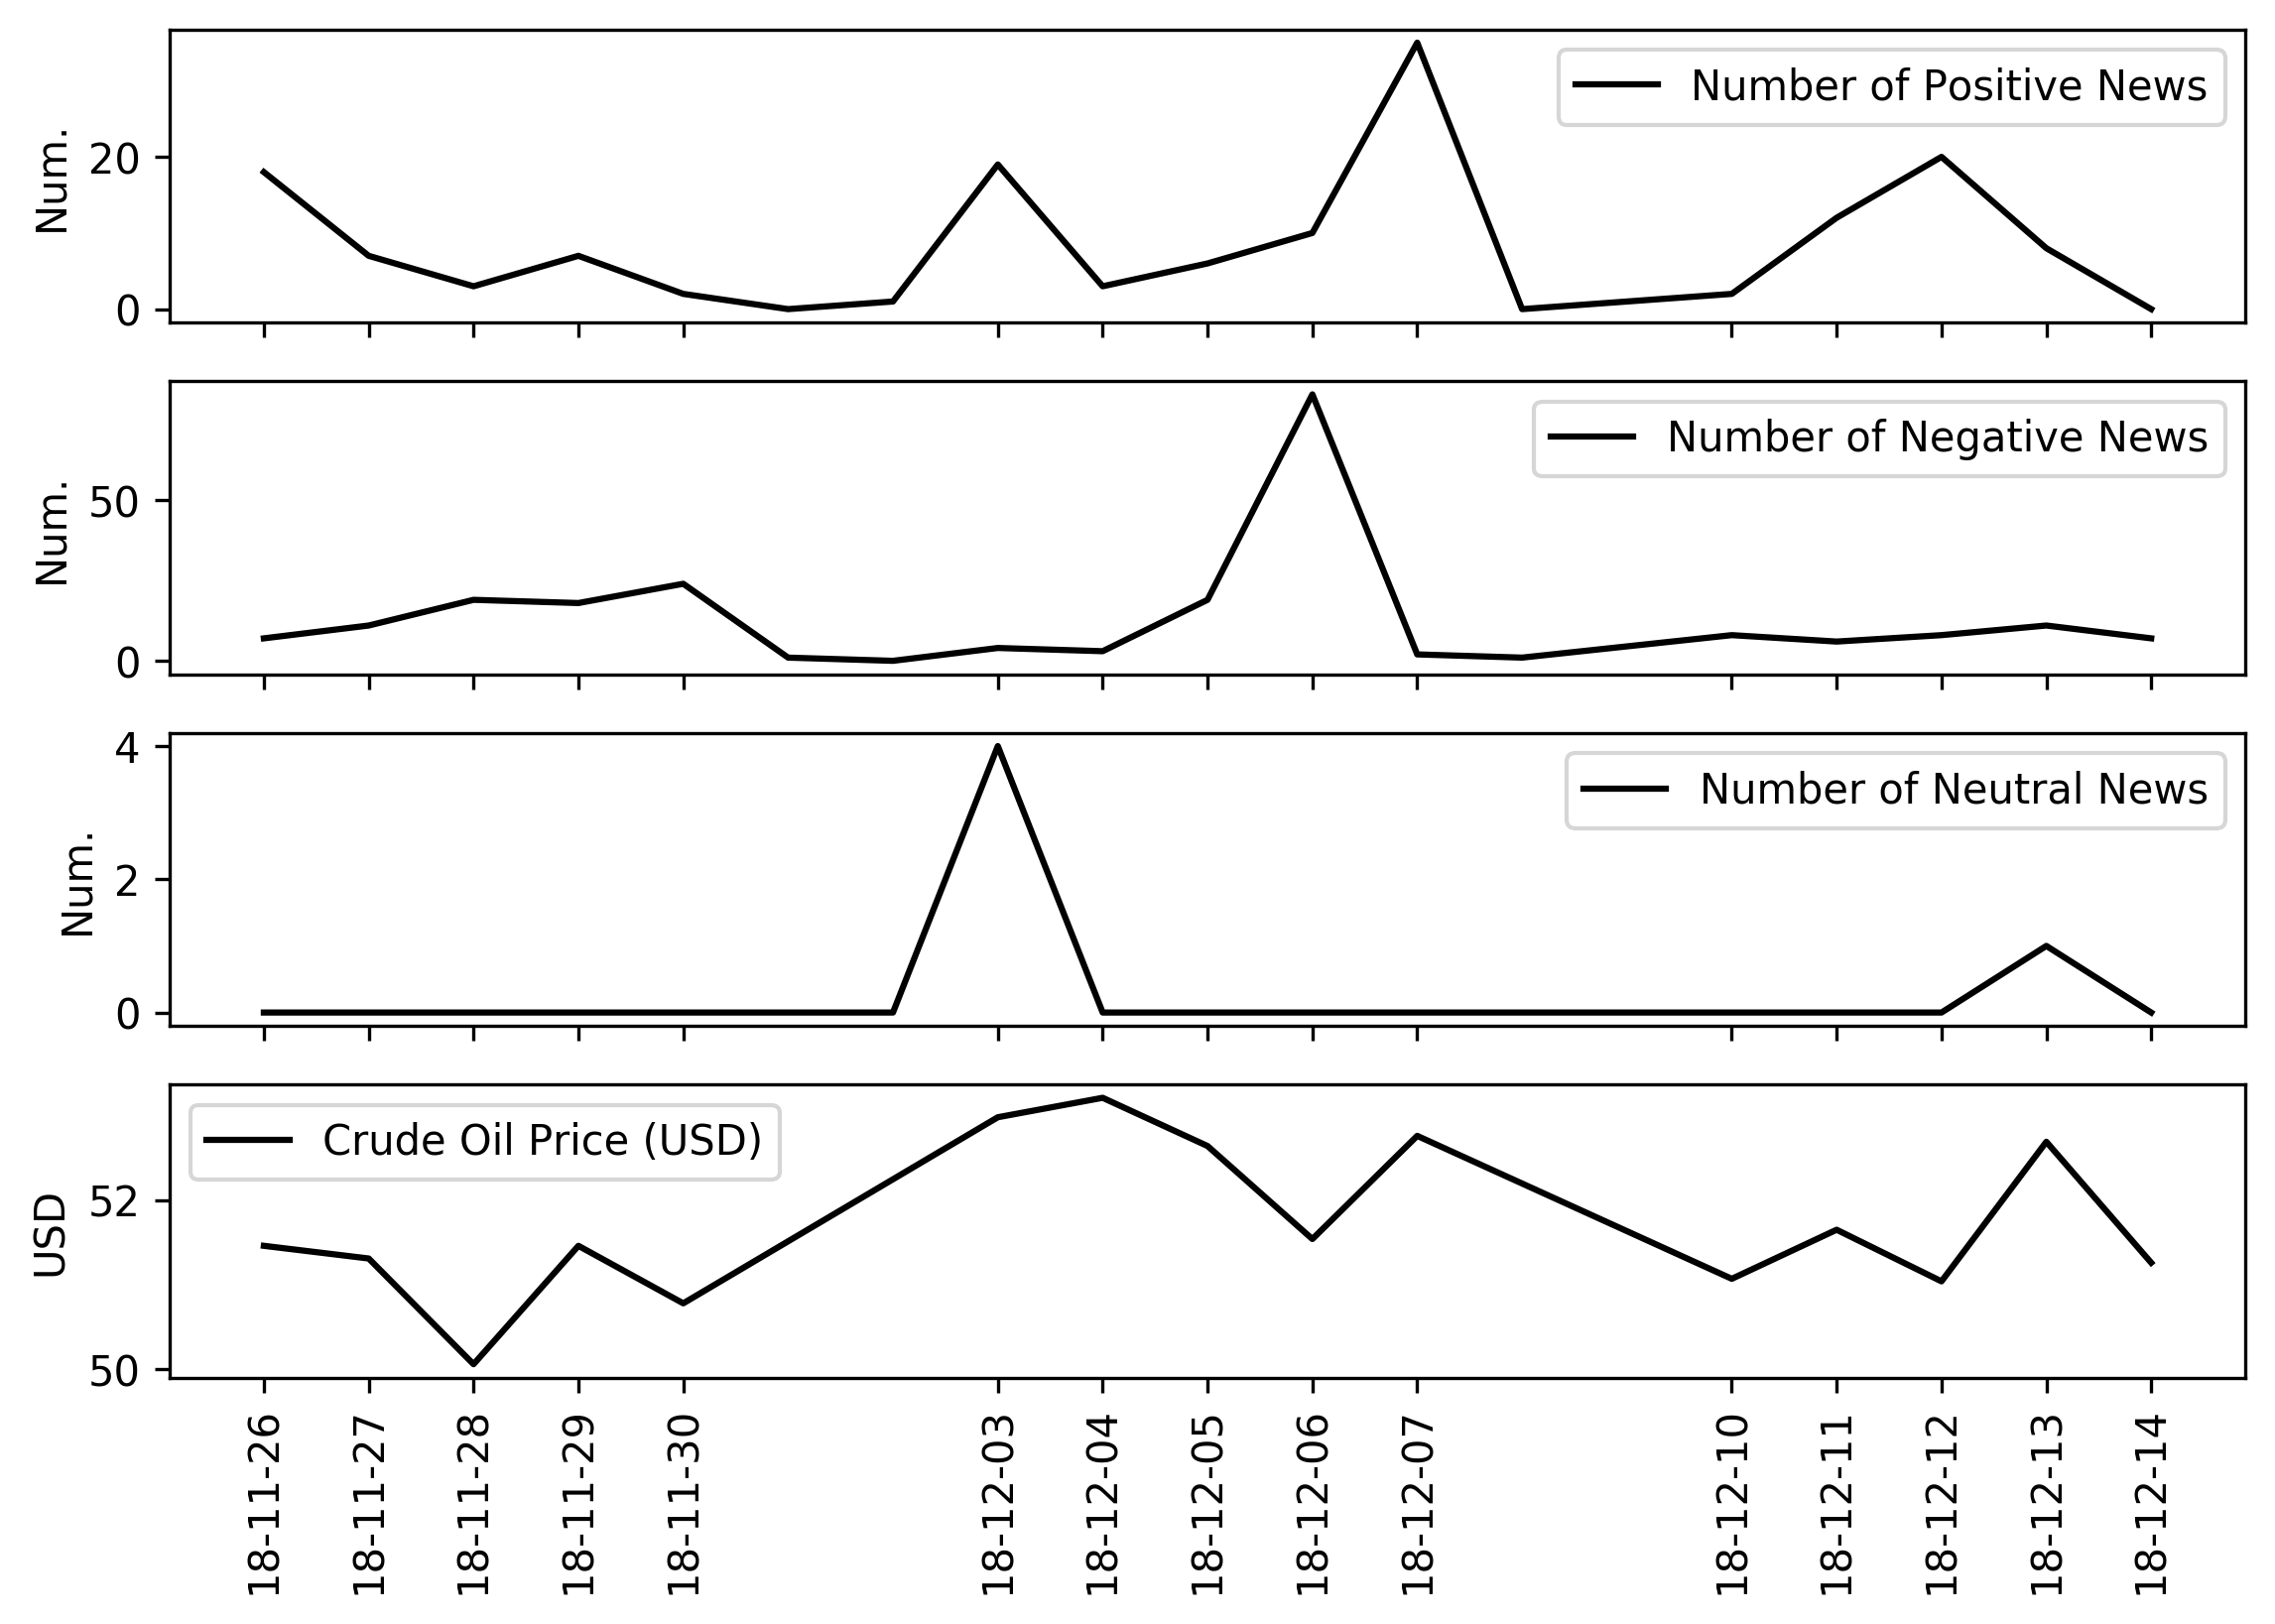
\includegraphics[width=\linewidth]{figures/case_studies/20181206_10d.png}
		\caption{}
	\end{figure}
	
	\subsubsection{Positive Spike on June. 12 - 13, 2019}
	\begin{figure}[H]
		\centering
		\small
		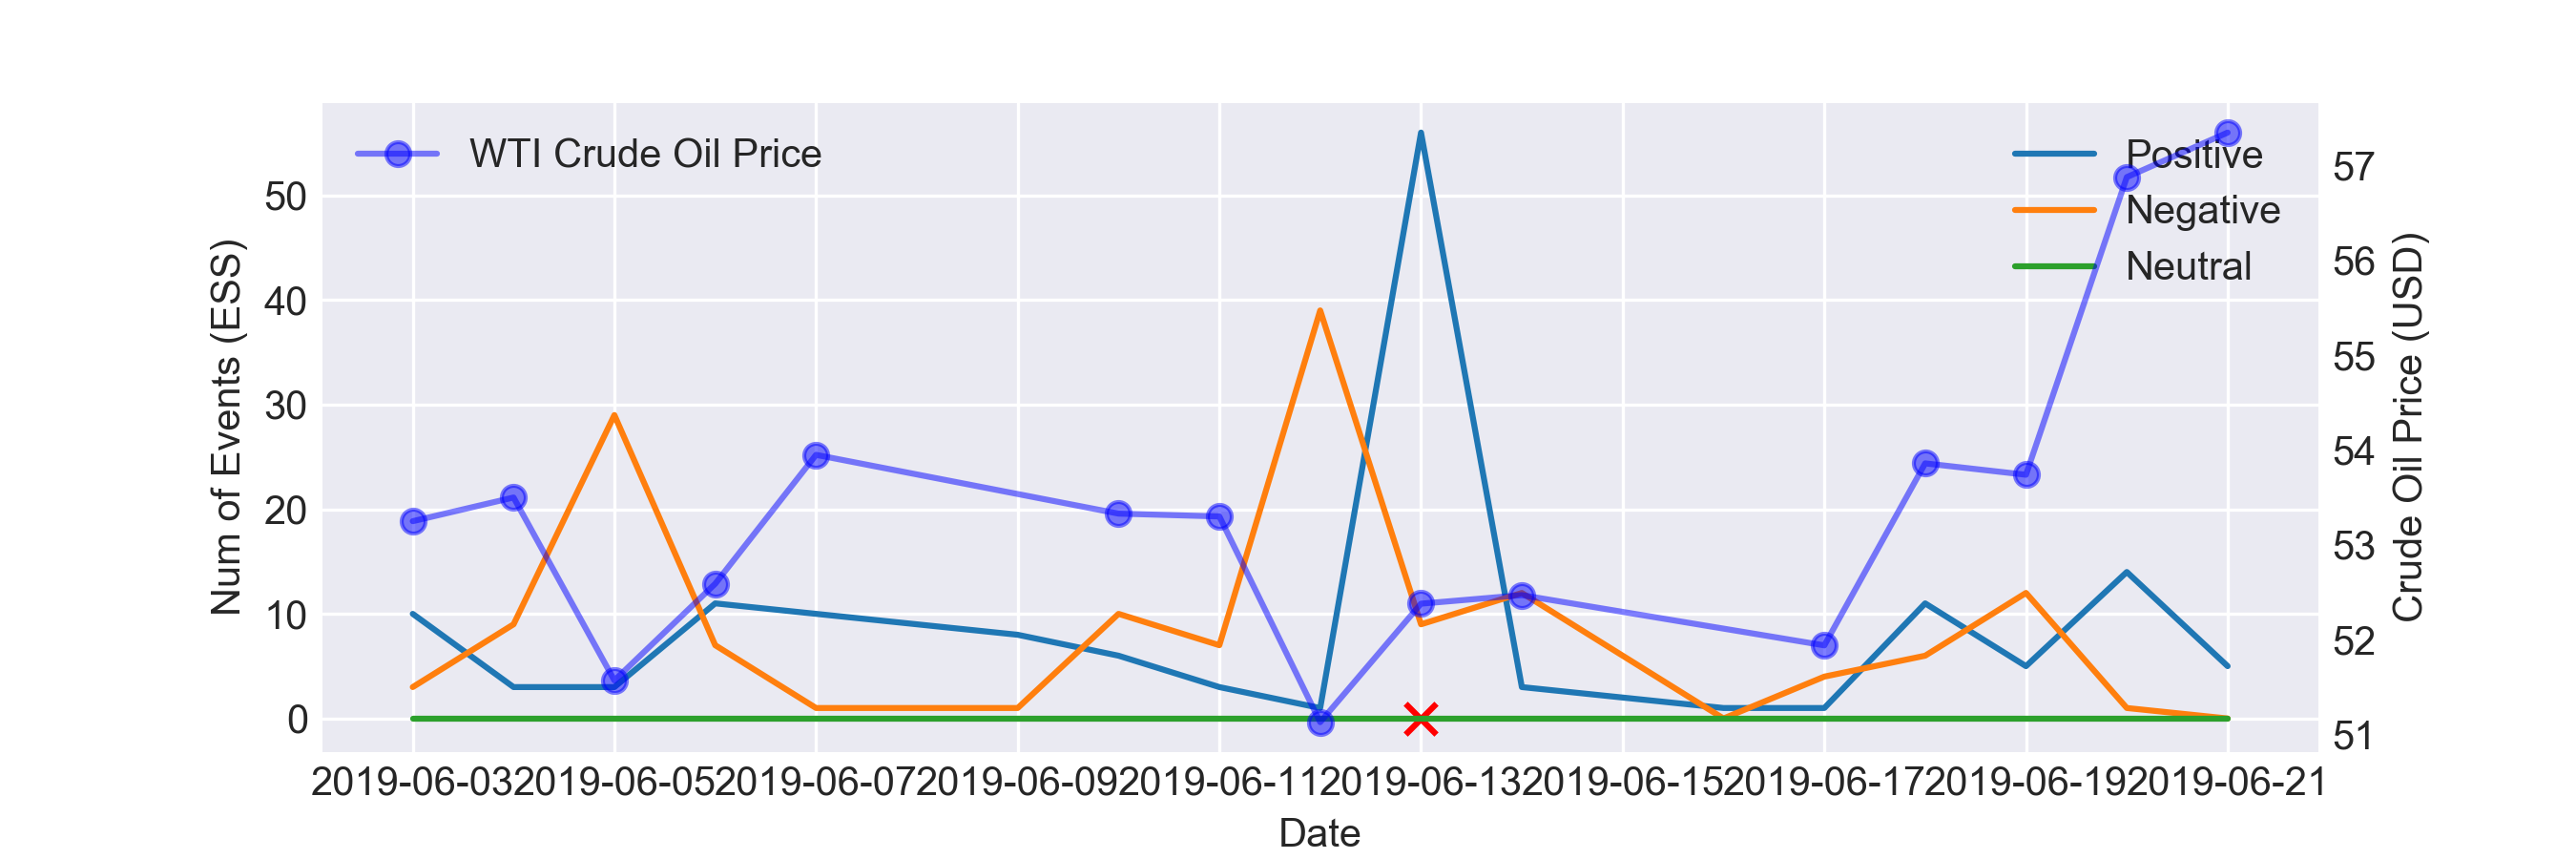
\includegraphics[width=\linewidth]{figures/case_studies/20190612_10d.png}
		\caption{}
	\end{figure}
	\section{Models}
	
	\section{Experiments}

	% Bib
	\bibliographystyle{apacite}
	
	\bibliography{thesis.bib}

	\section{Appendix: Supplementary Summary Statistics for Datasets}
	\begin{table}[H]
		\small
		\centering
		\begin{tabular}{l|c c c c c c c c c}
			\toprule
			Year & Num. Obs. & Mean & Median & Std. & Min & Max & ACF(1) & ACF(3) & ACF(5) \\
			\midrule
			2000 & 250 & 30.379 & 30.270 & 2.966 & 23.910 & 37.220 & 0.946 & 0.838 & 0.740 \\
			2001 & 250 & 25.983 & 27.185 & 3.560 & 17.500 & 32.210 & 0.973 & 0.924 & 0.880 \\
			2002 & 250 & 26.185 & 26.700 & 3.208 & 18.020 & 32.680 & 0.976 & 0.925 & 0.870 \\
			2003 & 250 & 31.075 & 30.770 & 2.624 & 25.250 & 37.960 & 0.943 & 0.864 & 0.764 \\
			2004 & 249 & 41.506 & 40.700 & 5.775 & 32.490 & 56.370 & 0.982 & 0.949 & 0.915 \\
			2005 & 251 & 56.637 & 57.330 & 6.252 & 42.160 & 69.910 & 0.969 & 0.917 & 0.876 \\
			2006 & 249 & 66.055 & 65.650 & 5.586 & 55.900 & 77.050 & 0.975 & 0.929 & 0.893 \\
			2007 & 252 & 72.341 & 69.735 & 12.853 & 50.510 & 99.160 & 0.986 & 0.956 & 0.924 \\
			2008 & 253 & 99.672 & 104.830 & 28.563 & 30.280 & 145.310 & 0.986 & 0.958 & 0.926 \\
			2009 & 252 & 61.950 & 67.025 & 13.361 & 34.030 & 81.030 & 0.985 & 0.959 & 0.928 \\
			2010 & 252 & 79.476 & 79.735 & 5.242 & 64.780 & 91.480 & 0.953 & 0.853 & 0.759 \\
			2011 & 252 & 94.881 & 95.790 & 8.063 & 75.400 & 113.390 & 0.968 & 0.900 & 0.828 \\
			2012 & 252 & 94.053 & 92.605 & 7.713 & 77.720 & 109.390 & 0.979 & 0.946 & 0.914 \\
			2013 & 252 & 97.983 & 96.325 & 5.451 & 86.650 & 110.620 & 0.977 & 0.927 & 0.881 \\
			2014 & 252 & 93.172 & 97.850 & 13.519 & 53.450 & 107.950 & 0.978 & 0.936 & 0.895 \\
			2015 & 252 & 48.657 & 47.870 & 6.814 & 34.550 & 61.360 & 0.972 & 0.928 & 0.888 \\
			2016 & 252 & 43.294 & 45.080 & 6.727 & 26.190 & 54.010 & 0.978 & 0.932 & 0.893 \\
			2017 & 250 & 50.800 & 50.385 & 3.914 & 42.480 & 60.460 & 0.968 & 0.905 & 0.846 \\
			2018 & 249 & 65.227 & 66.380 & 6.517 & 44.480 & 77.410 & 0.961 & 0.888 & 0.812 \\
			2019 & 187 & 57.037 & 56.580 & 3.986 & 46.310 & 66.240 & 0.924 & 0.811 & 0.732 \\
			\midrule
			Total & 4956 & 61.956 & 58.915 & 26.376 & 17.500 & 145.310 & 0.998 & 0.995 & 0.992 \\
			\bottomrule
		\end{tabular}
		\caption{Summary Statistics for Crude Oil Prices. Note that this dataset only include nine months of 2019.}
	\end{table}
	
	\begin{figure}[H]
		\centering
		\small
		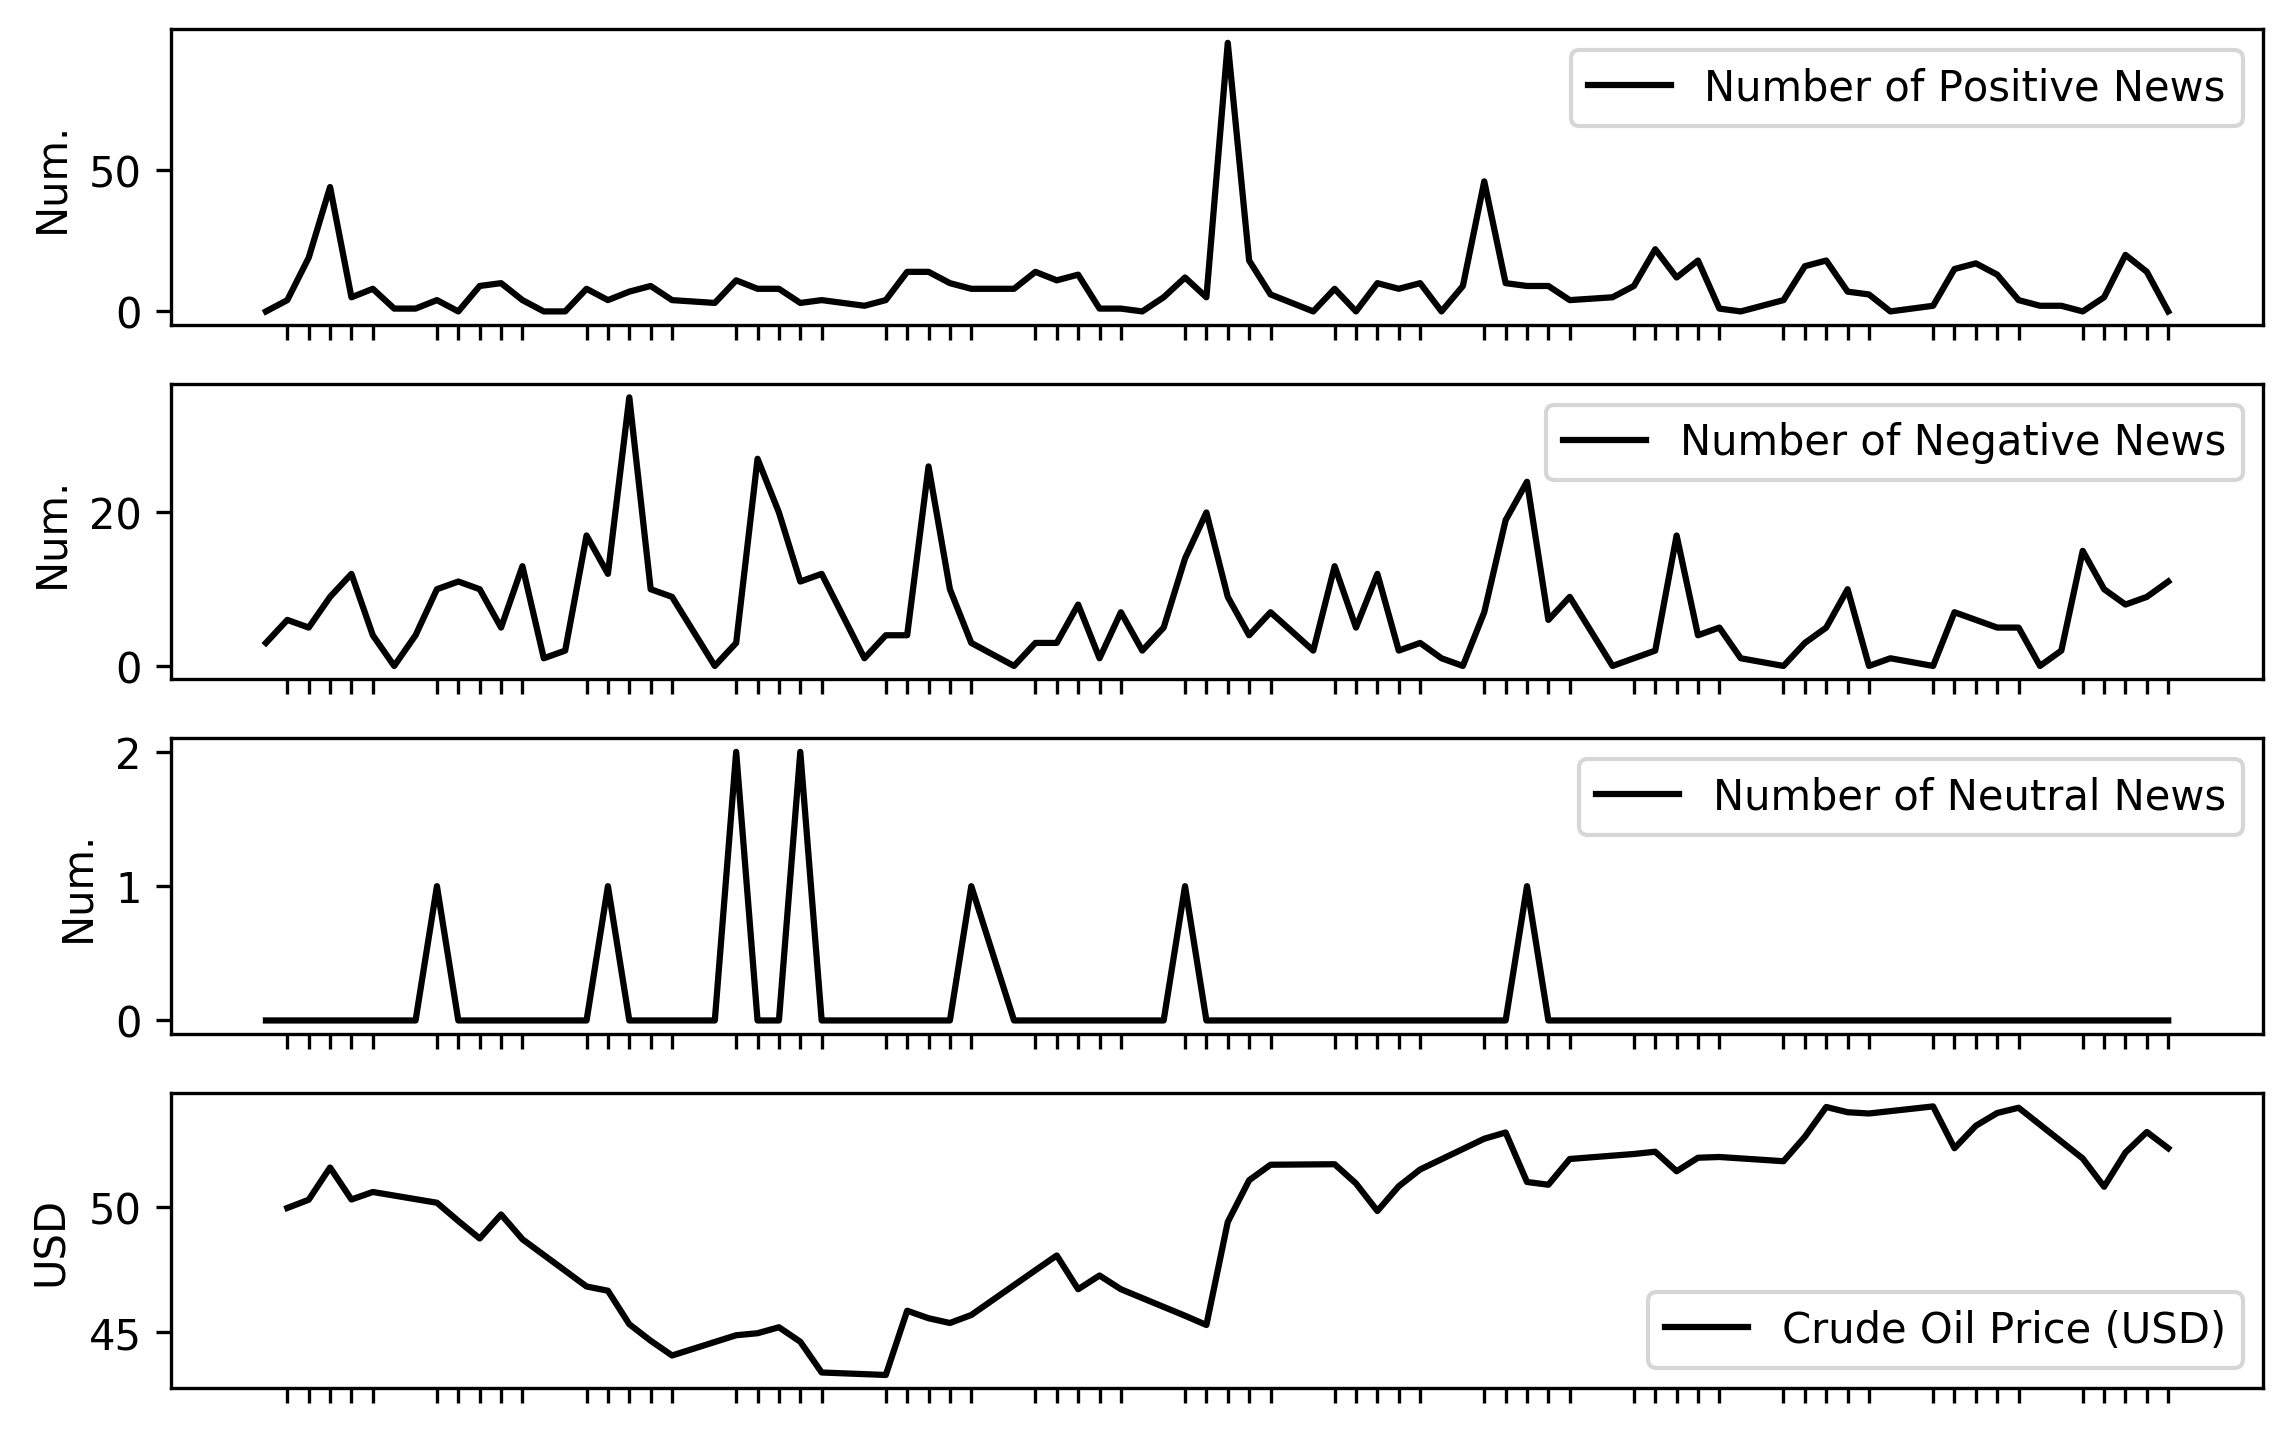
\includegraphics[width=\linewidth]{figures/case_studies/20161130_45d.png}
		\caption{}
	\end{figure}
	\begin{figure}[H]
		\centering
		\small
		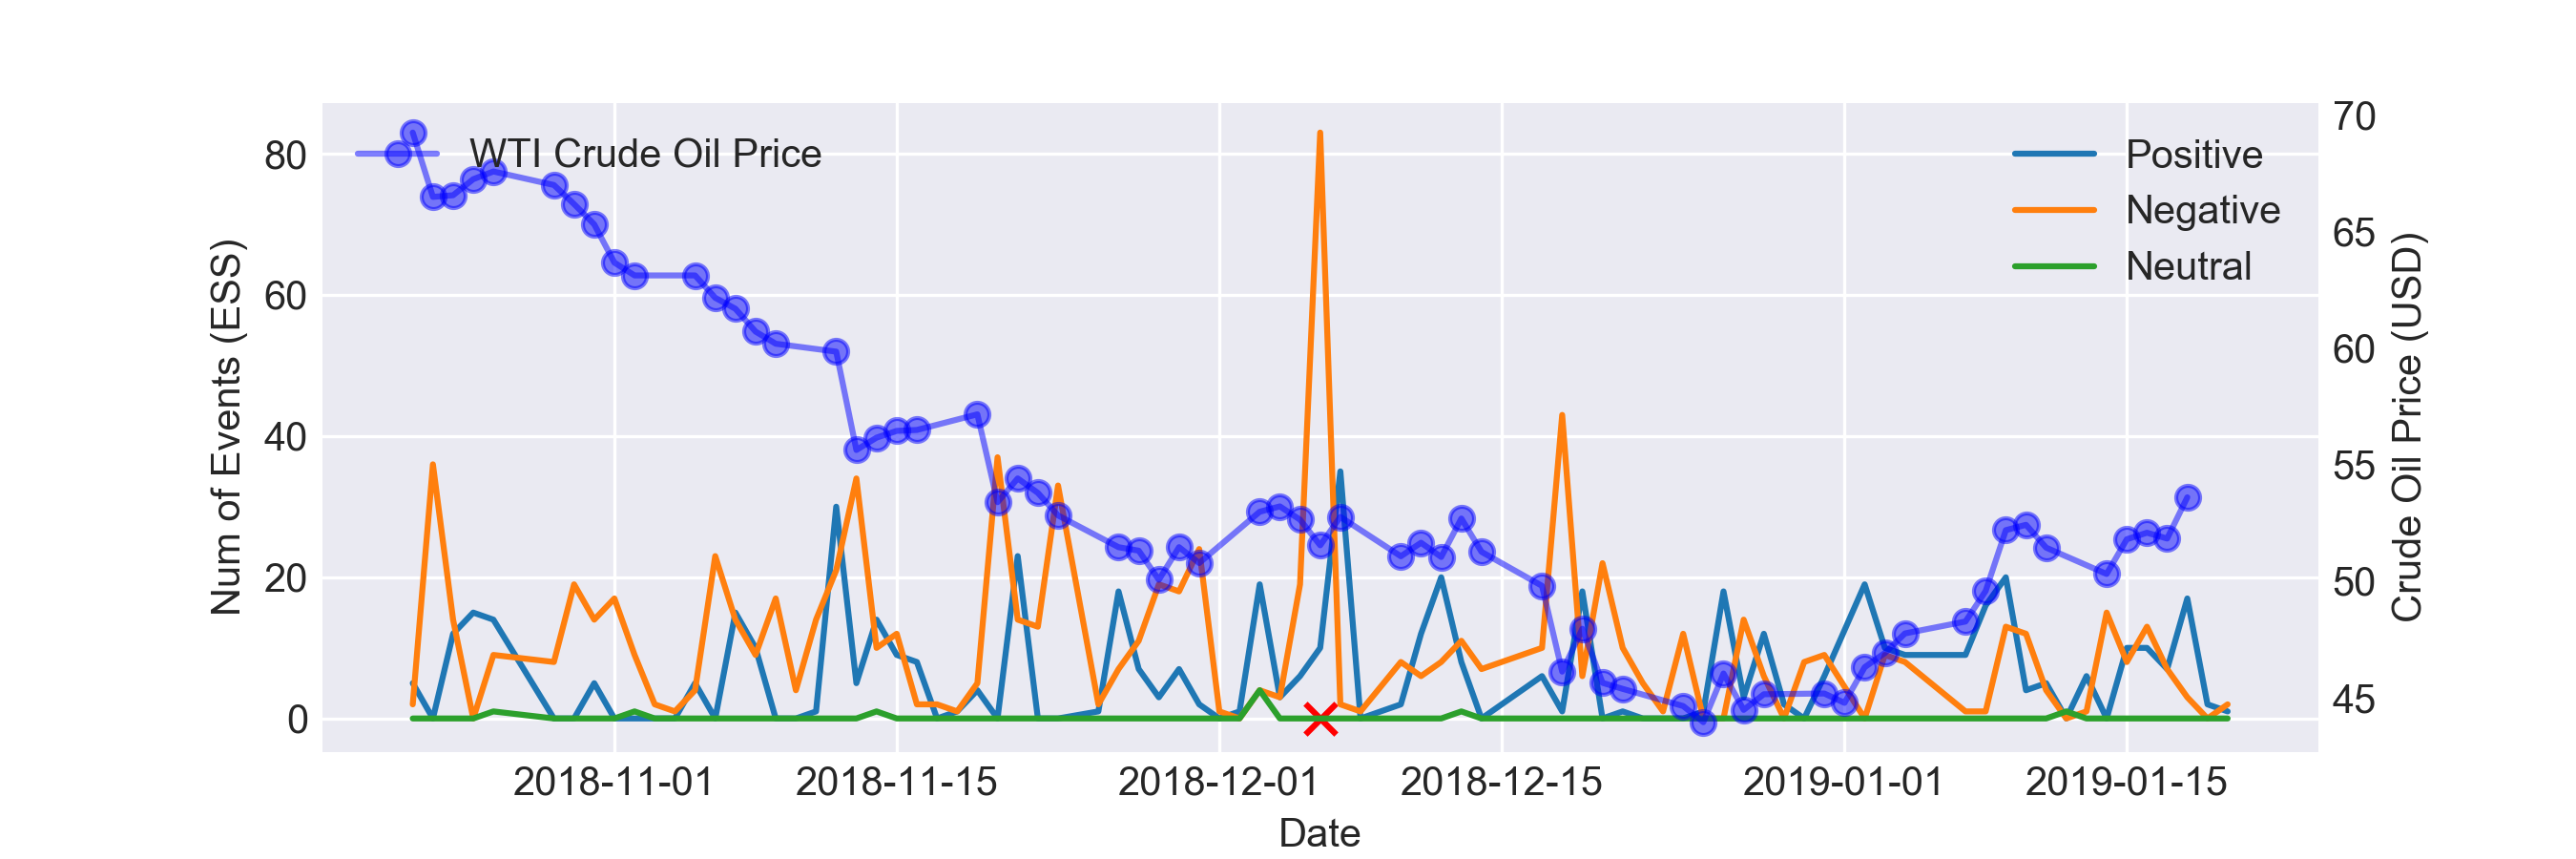
\includegraphics[width=\linewidth]{figures/case_studies/20181206_45d.png}
		\caption{}
	\end{figure}
	\begin{figure}[H]
		\centering
		\small
		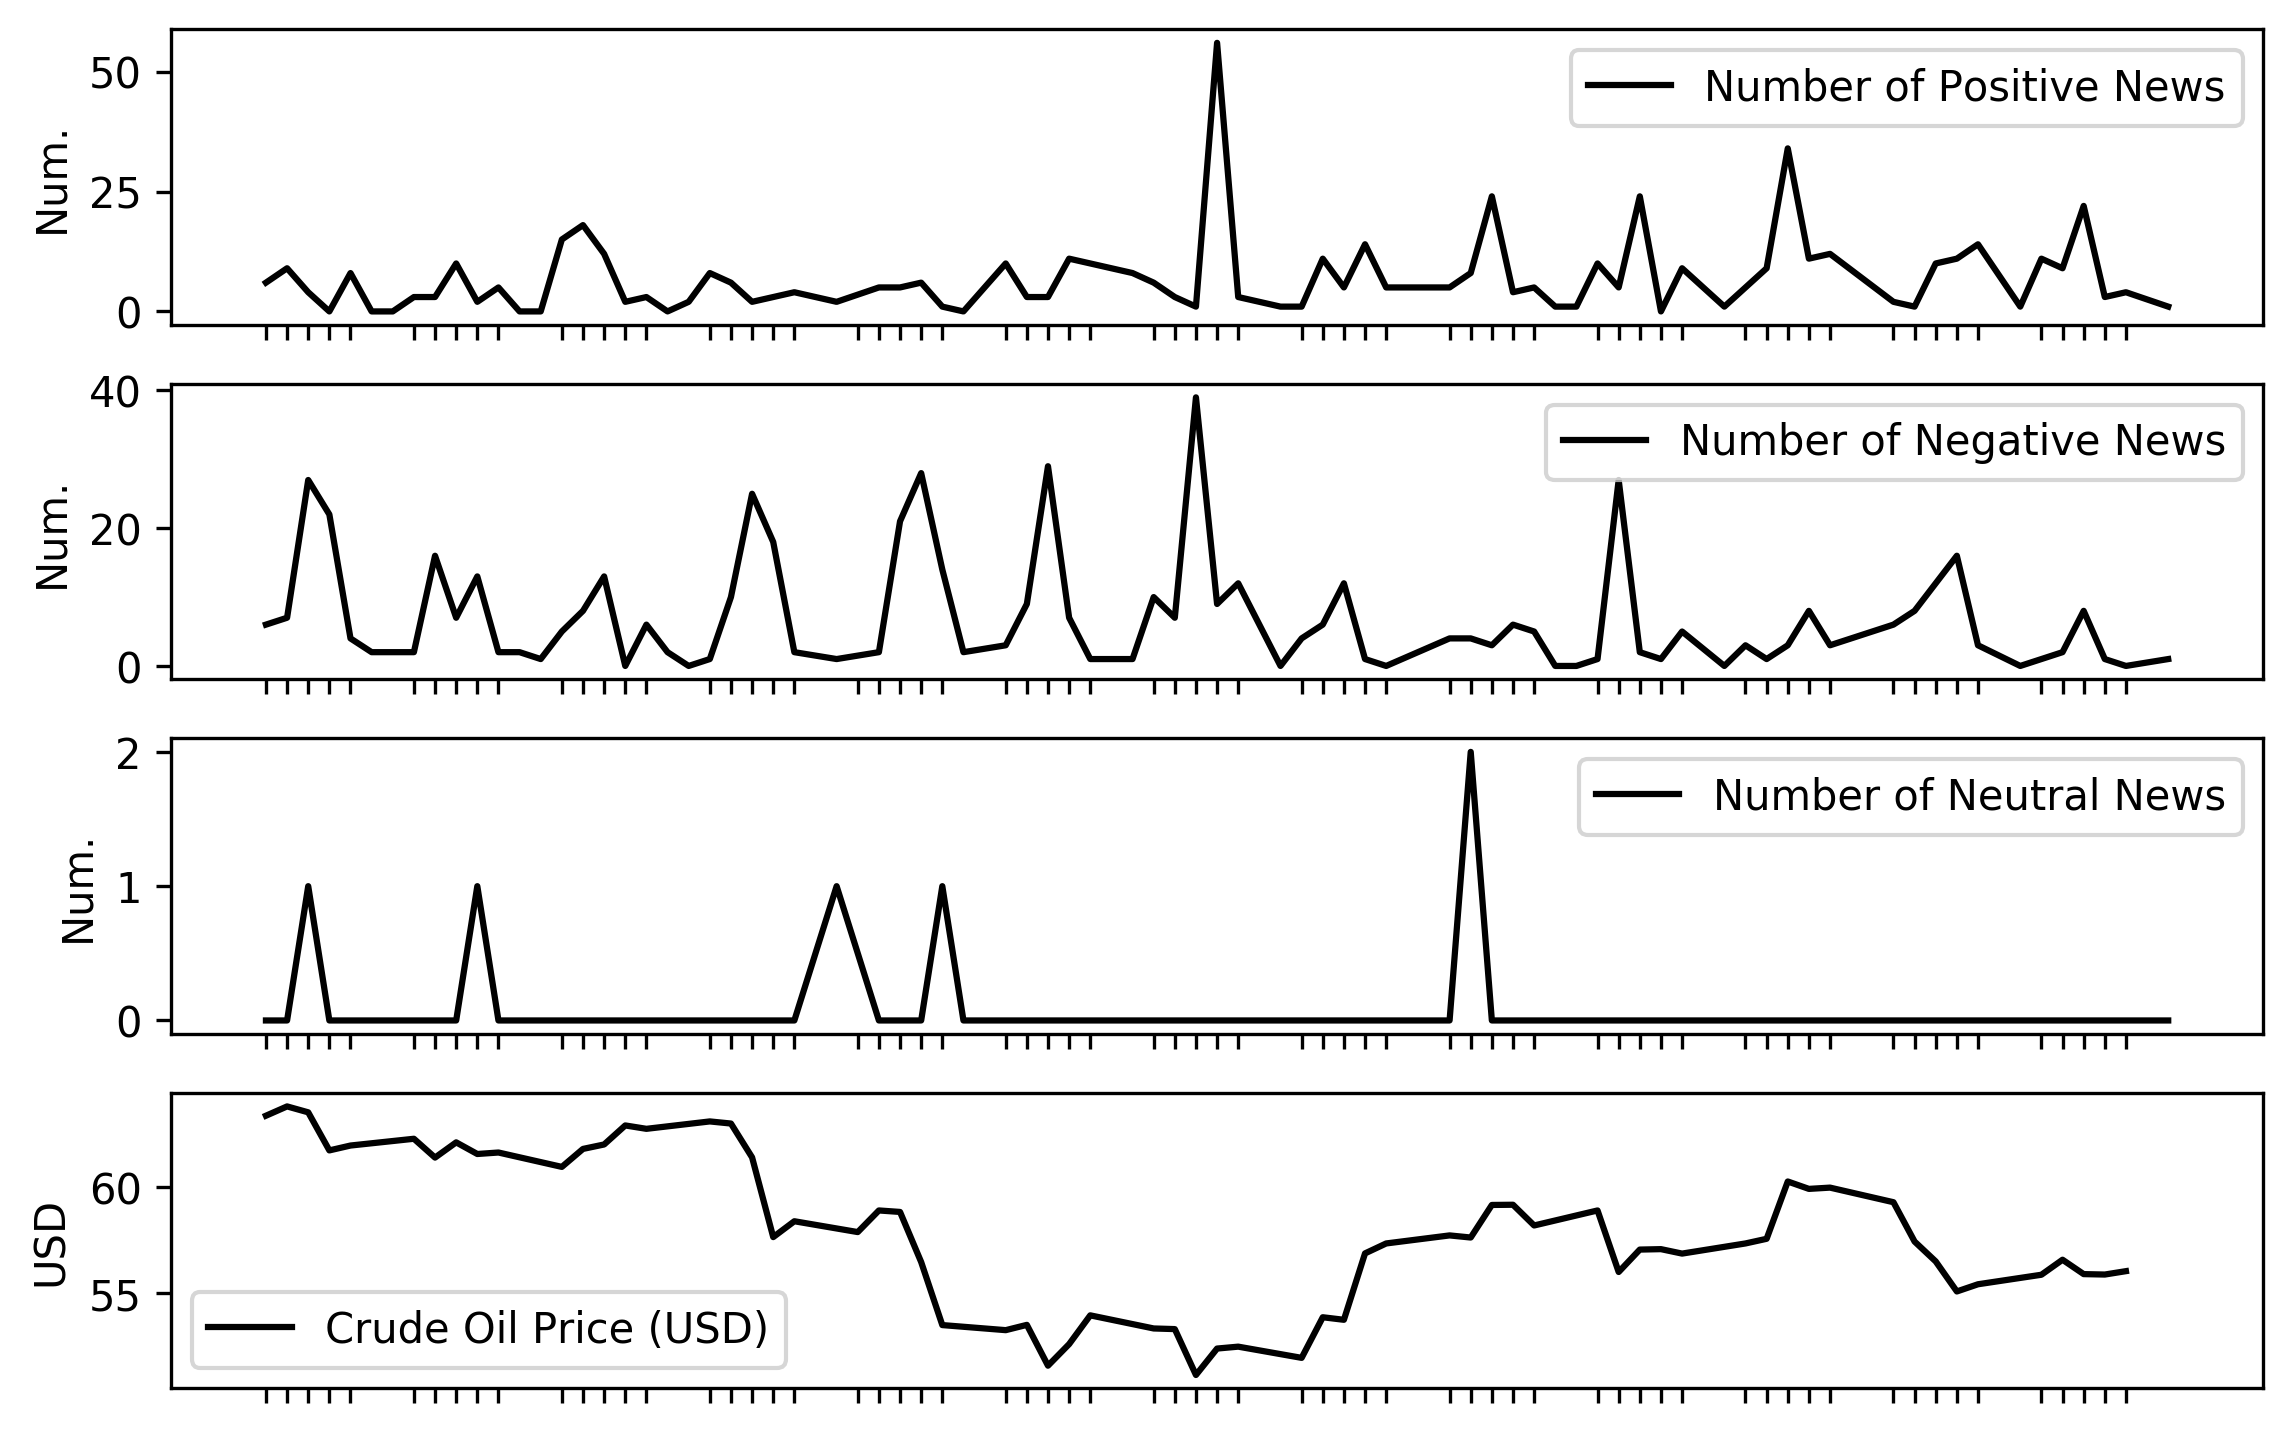
\includegraphics[width=\linewidth]{figures/case_studies/20190612_45d.png}
		\caption{}
	\end{figure}
\end{document}






















